\chapter{Results and Analysis} 
%Created 21-12-2016 (04-03-2016 first) 
\label{ch:results}
With the program validated, both case 1 and case 2 can be used to examine the behaviour of \ac{TSI}. This is done in a sensitivity analysis and is very useful to determine the limitations and characteristics of this method. In the previous chapter the trajectories from both \ac{TSI} and \ac{RKF} were plotted and it could be seen that the results were very similar to the point where the accuracy of \ac{TSI} was validated. Therefore, in this chapter the performance of \ac{TSI} will be compared to \ac{RKF} to determine any advantages and disadvantages. In order to do this only one variable will be changed every time, which means that from the nominal case only one parameter will be different. This way the effects can be clearly associated with that particular parameter, which provides a solid base of comparison. The nominal values for both the first and second case are provided in \Cref{app:appendixF-nominalCaseInputValues}. It is also important to have the same cut-off point. This can either be a certain altitude, set end time or zero degrees flight-path angle. Usually the set end time is taken as the cut-off criteria to determine the difference in state. Sometimes the altitude is used in cases where it is interesting to see when a certain altitude is reached and under what conditions when a certain parameter is changed. An example was shown in the validation chapter where certain conditions had to be met at a certain altitude. And in some cases it is best to set the zero degrees flight-path angle as a cut-off criteria because either the cut-off time or altitude will never be reached but the effects of a parameter still need to be investigated. This last cut-off criteria is the "fail-safe" for every simulation because this prevents the simulation from going back to the surface and literally crashing the program. In this chapter every section discusses the effect of a different parameter or focusses on one aspect of the simulation. \\

Besides comparing \ac{TSI} to \ac{RKF} it will also be compared to the non-rotational case. The nominal case takes the rotating Mars into account, however it is interesting to see what \ac{TSI} does when the rotation is turned off. For these two cases to be properly compared, again for most parameters, the set end time is the cut-off criteria unless mentioned otherwise.\\

The parameters changed in this sensitivity analysis are: order, error tolerance, launch altitude, launch latitude, launch longitude, flight-path angle and heading angle. A multiple run analysis will also be described where the nominal case is run for a number of times and the CPU time is compared. 


\section{Order}
\label{sec:order}
For most classic integrators the order is set and cannot be easily changed. For \ac{RKF} for instance, a whole new set of coefficients is required if a different order is desired. However, for \ac{TSI} changing the order is as simple as updating the maximum order input value. Theoretically this means that an infinite order can be chosen to get the most accurate result. The question is, is this indeed the most optimal. \Cref{subsec:optimalOrder} hopes to answer this question by looking at the CPU time. In \Cref{subsec:orderCompNotRot} a range of orders has been run for both cases. Once with the nominal conditions of a rotating Mars and once assuming a non-rotating Mars. The effect of the rotating Mars will be investigated. The cut-off criteria for case 1 was an end time of 1796 seconds for the data collection case and 789 seconds without live data collection. For case 2 the cut-off criteria was 876 second for both runs.

\subsection{Optimal order}
\label{subsec:optimalOrder}
To determine the optimal order an important criteria is that the outcome is accurate, however, what is often more important is that this accurate outcome is computed really fast. This is why, in order to find the optimum order, the CPU time is the most important criteria. In order to properly observe the effect of a different order, the nominal case is run for different orders. Thus the only difference will be the maximum order. This can be done for the two presented cases. During real-life simulations a user can choose to either collect all the data during the simulation or only store the final outcomes at the end of the simulation. Storing data during the integration requires a lot of computational power and will therefore increase the CPU time required, but this will provide the user with the desired trajectory data. Both cases with and without live data collection have been run for a specific range of orders depending on the case, and the results are shown in \Cref{fig:orderVsCPUcase1IncludingLiveDataCollection}.
The first case was run with a maximum order ranging from 5 to 100, and the second case was run from 5 to 31 because of the behaviour observed during the first case runs. 



\begin{figure}[H]
\centering
\subfloat[]{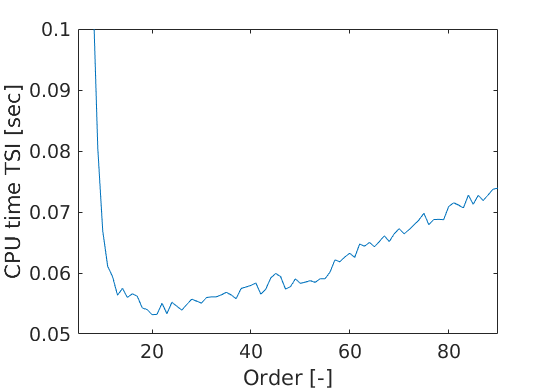
\includegraphics[width=3.1in]{figures/results/Order/orderVsCPUcase1IncludingLiveDataCollection.png}\label{subfig:orderVsCPUcase1IncludingLiveDataCollection}} 
\subfloat[]{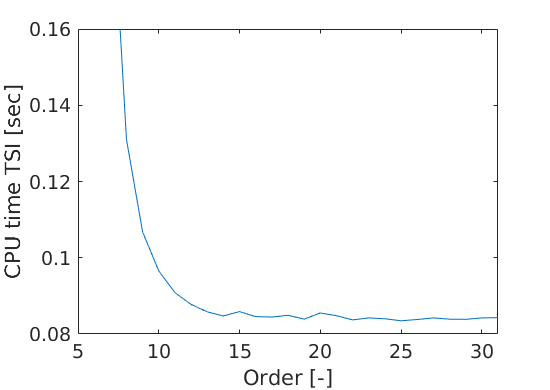
\includegraphics[width=3.1in]{figures/results/Order/orderVsCPUcase2IncludingLiveDataCollection.png} \label{subfig:orderVsCPUcase2IncludingLiveDataCollection}}\\
 
\subfloat[]{\includegraphics[width=3.1in]{figures/results/Order/orderVsCPUcase1NoDataCollection.png}\label{subfig:orderVsCPUcase1NoDataCollection}} 
\subfloat[]{\includegraphics[width=3.1in]{figures/results/Order/orderVsCPUcase2NoDataCollection.png}\label{subfig:orderVsCPUcase2NoDataCollection}}
\caption{Order versus CPU time \protect\subref{subfig:orderVsCPUcase1IncludingLiveDataCollection} case 1 including live data collection, \protect\subref{subfig:orderVsCPUcase2IncludingLiveDataCollection} case 2 including live data collection, \protect\subref{subfig:orderVsCPUcase1NoDataCollection} case 1 without live data collection, \protect\subref{subfig:orderVsCPUcase2NoDataCollection} case 2 without live data collection } 
\label{fig:orderVsCPUcase1IncludingLiveDataCollection} 
\end{figure} 

Looking at \Cref{subfig:orderVsCPUcase1IncludingLiveDataCollection} it is clear that the order versus CPU curve can be split up into two phases that have different properties that influence the CPU time. The first phase shows a rapid decrease in the CPU time until order 20 is reached, the second phase continues from that point until the final order is reached. The order has a direct relation to the chosen step-size that \ac{TSI} computes automatically because the step-size is determined by the error tolerance and the difference between the penultimate Taylor Series coefficient and the final one (as described in \Cref{subsec:stepSizeTsi}). This means that if these last two coefficients show a large difference, which can happen lower order because fewer derivatives are taken into account, the step-size will be lowered and thus increasing the number of steps. In the first phase, this large number of steps result in a high CPU time. Another factor that affects the CPU time is the number of derivatives taken into account, which is directly related to the order (10 as maximum order equals 10 derivatives that are taken into account). At a certain point, an increase in order does not affect the number of steps that much any more, resulting in a decrease of 3 to 1 steps with every order increase. The result is that the number of steps remains approximately the same but the number of derivatives that are taken into account keeps increasing. Every extra derivative means an extra computation per auxiliary equation/variable. This is what is observed in the second phase. Here the effect of adding more computations on the CPU time becomes clear, showing a corresponding increase in CPU time. This tipping point between the two phases can be observed around the lowest CPU time, where the effect of the number of steps and the number of derivative computations equal out. This is therefore the optimum order for the \ac{TSI} method. The two phases can be observed in each of the four graphs, however, because the increase of CPU time, the higher orders were not required and were thus left out in the simulations for case 2. For each of the simulation runs, the two orders which resulted in the lowest CPU time have been recorded in \Cref{tab:orderAndCPUtimes}. 

\begin{table}[H]
\begin{center}
\caption{Lowest two orders with corresponding CPU times for each of the sub-graphs}
\label{tab:orderAndCPUtimes}
\begin{tabular}{|l|l|l|l|l|}
\hline 
\textbf{Sub-graph}  & \multicolumn{2}{c|}{\textbf{Lowest CPU time}} & \multicolumn{2}{c|}{\textbf{Second lowest CPU time}} \\ \cline{2-5}

& \textbf{Order} &
\textbf{CPU time [s]} & \textbf{Order} & \textbf{CPU time [s]} \\ \hline \hline

a & 20 & 0.053162 & 21 & 0.053226 \\ \hline
b & 25 & 0.083474 & 22 & 0.0837 \\ \hline
c & 14 & 0.007465 & 20 & 0.007736 \\ \hline
d & 18 & 0.008273 & 20 & 0.008314 \\ \hline


\end{tabular}
\end{center}
\end{table}

In the table and the graphs it can be seen that the minima are all situated around an order of 20, which is why a maximum order of 20 was set as the nominal value and used for all simulations.

%a: 20 = 0.053162 s, 21 = 0.053226 s
%b: 25 = 0.083474 s, 22 = 0.0837 s
%c: 14 = 0.007465 s, 20 = 0.007736 s
%d: 18 = 0.008273 s, 20 = 0.008314 s

%Show both plots of orders and then talk about the fastest order and explain what you can see. First part of graph is the number of evaluations important and last part is the amount of computations that have to be made because the number of evaluations don't change any more.
%
%Graphs needed:
%
%- CPU time vs order case 1 and case 2


% \begin{figure}[H]
%\centering
%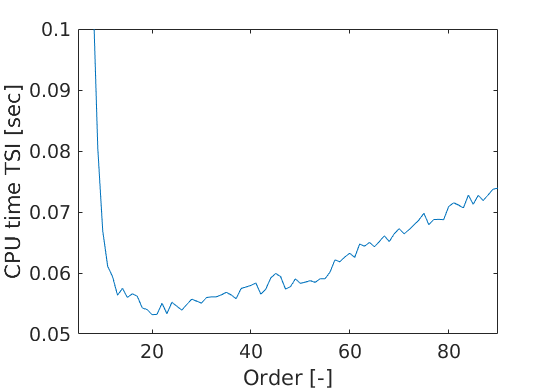
\includegraphics[width=0.7\textwidth]{figures/results/Order/orderVsCPUcase1IncludingLiveDataCollection.png}
%\caption{Order versus CPU time case 1 including live data collection.}
%\label{fig:orderVsCPUcase1IncludingLiveDataCollection}
%\end{figure}

%\begin{figure}
%\centering
%\subfloat[]{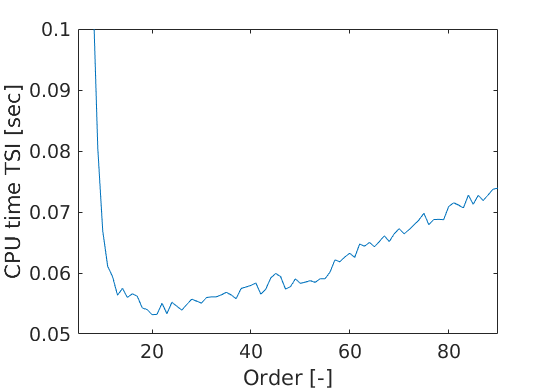
\includegraphics[width=3.1in]{figures/results/Order/orderVsCPUcase1IncludingLiveDataCollection.png}\label{subfig:orderVsCPUcase1IncludingLiveDataCollection}} 
%\subfloat[]{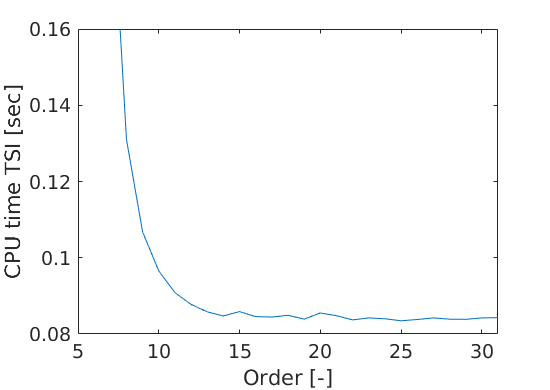
\includegraphics[width=3.1in]{figures/results/Order/orderVsCPUcase2IncludingLiveDataCollection.png}\label{subfig:orderVsCPUcase2IncludingLiveDataCollection}}
%\caption{Order versus CPU time including live data collection \protect\subref{subfig:orderVsCPUcase1IncludingLiveDataCollection} case 1 \protect\subref{subfig:orderVsCPUcase2IncludingLiveDataCollection} case 2 } 
%\label{fig:orderVsCPUcase1IncludingLiveDataCollection} 
%\end{figure} 
%
%\begin{figure}
%\centering
%\subfloat[]{\includegraphics[width=3.1in]{figures/results/Order/orderVsCPUcase1NoDataCollection.png}\label{subfig:orderVsCPUcase1NoDataCollection}} 
%\subfloat[]{\includegraphics[width=3.1in]{figures/results/Order/orderVsCPUcase2NoDataCollection.png}\label{subfig:orderVsCPUcase2NoDataCollection}}
%\caption{Order versus CPU time without live data collection \protect\subref{subfig:orderVsCPUcase1NoDataCollection} case 1 \protect\subref{subfig:orderVsCPUcase2NoDataCollection} case 2 } 
%\label{fig:orderVsCPUcase1NoDataCollection} 
%\end{figure} 

%Tables needed:
%
%- Zoom in numbers around Order 20 to prove it is the fastest \\

\subsection{Comparison with non-rotating Mars}
\label{subsec:orderCompNotRot}
For the comparison of the rotating and the non-rotating cases with a varying order it is again interesting to look at the differences in CPU time. \Cref{fig:orderVsCPUcase1combined} shows these plots for both cases when the trajectory data is not collected during the simulation. It can be seen that for case 1, on average, the non-rotating runs are faster. Also, for a non-rotating Mars the optimum order is 20 as well. The difference in CPU time is better shown by the case 2 run, where the non-rotating curve fits perfectly below the rotating curve. Here, the order 20 has again the second lowest CPU time (the lowest is order 17 with a time difference of 28 microseconds). The time difference between the curves of the rotating and non-rotating Mars can be explained by the fact that if Mars does not rotate, the rotating effects become zero, which reduces the number of computations.
%Explain what you can see in the graph and why that is probably the case.
%
%Graphs needed:
%
%- CPU time vs order case 1 combined \\
%- CPU time vs order case 2 combined \\
%
%
%- RKF difference in end state before circularisation combined case 1 \\ 
%- RKF difference in end state before circularisation combined case 2 \\
%- Consecutive difference in end state before cicularisation combined case 1 \\
%- Consecutive difference in end state before cicularisation combined case 2 \\
%- Nominal case difference in end state before circularisation combined case 1 \\
%- Nominal case difference in end state before circularisation combined case 2 \\
%


\begin{figure}[H]
\centering
\subfloat[]{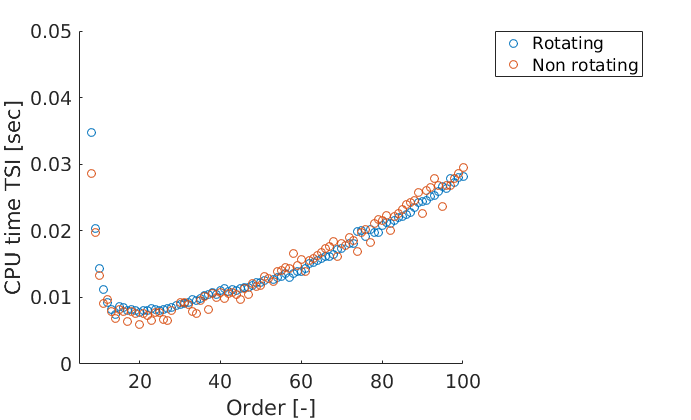
\includegraphics[width=3.1in]{figures/results/Order/orderVsCPUcase1combined.png}\label{subfig:orderVsCPUcase1combined}} 
\subfloat[]{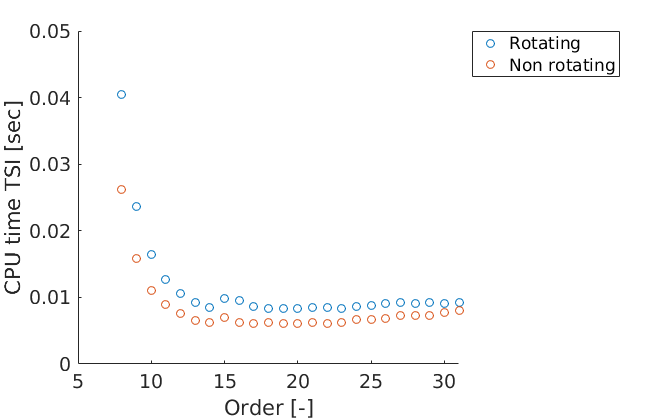
\includegraphics[width=3.1in]{figures/results/Order/orderVsCPUcase2combined.png}\label{subfig:orderVsCPUcase2combined}}
\caption{Order versus CPU time for rotating and non-rotating Mars \protect\subref{subfig:orderVsCPUcase1combined} case 1,  \protect\subref{subfig:orderVsCPUcase2combined} case 2 } 
\label{fig:orderVsCPUcase1combined} 
\end{figure} 

As was mentioned before, the accuracy of  the results is very important. In \Cref{fig:orderVsRKFAbsoluteDifferenceCase1combined} the absolute difference between the nominal end state of \ac{RKF} before circularisation and \ac{TSI} for both the rotating and non-rotating Mars. A trend can be identified where it is shown that an order of 11 or higher will result in a difference of $\mu$m in position and nm/s in velocity. Even the lowest order of 5 results in an accuracy of less than 10 cm for position and 10 mm/s for velocity. The spikes in the first case are caused by a slight error resulting from the combination of variables that result at those specific orders. This proves that the simulator is not yet robust enough and could still use some improvements. One improvement that might solve this problem is a change in the manner in which the step-size is computed. Additional comparison plots are shown in \Cref{app:appendixG-Results}.

\begin{figure}[H]
\centering
\subfloat[]{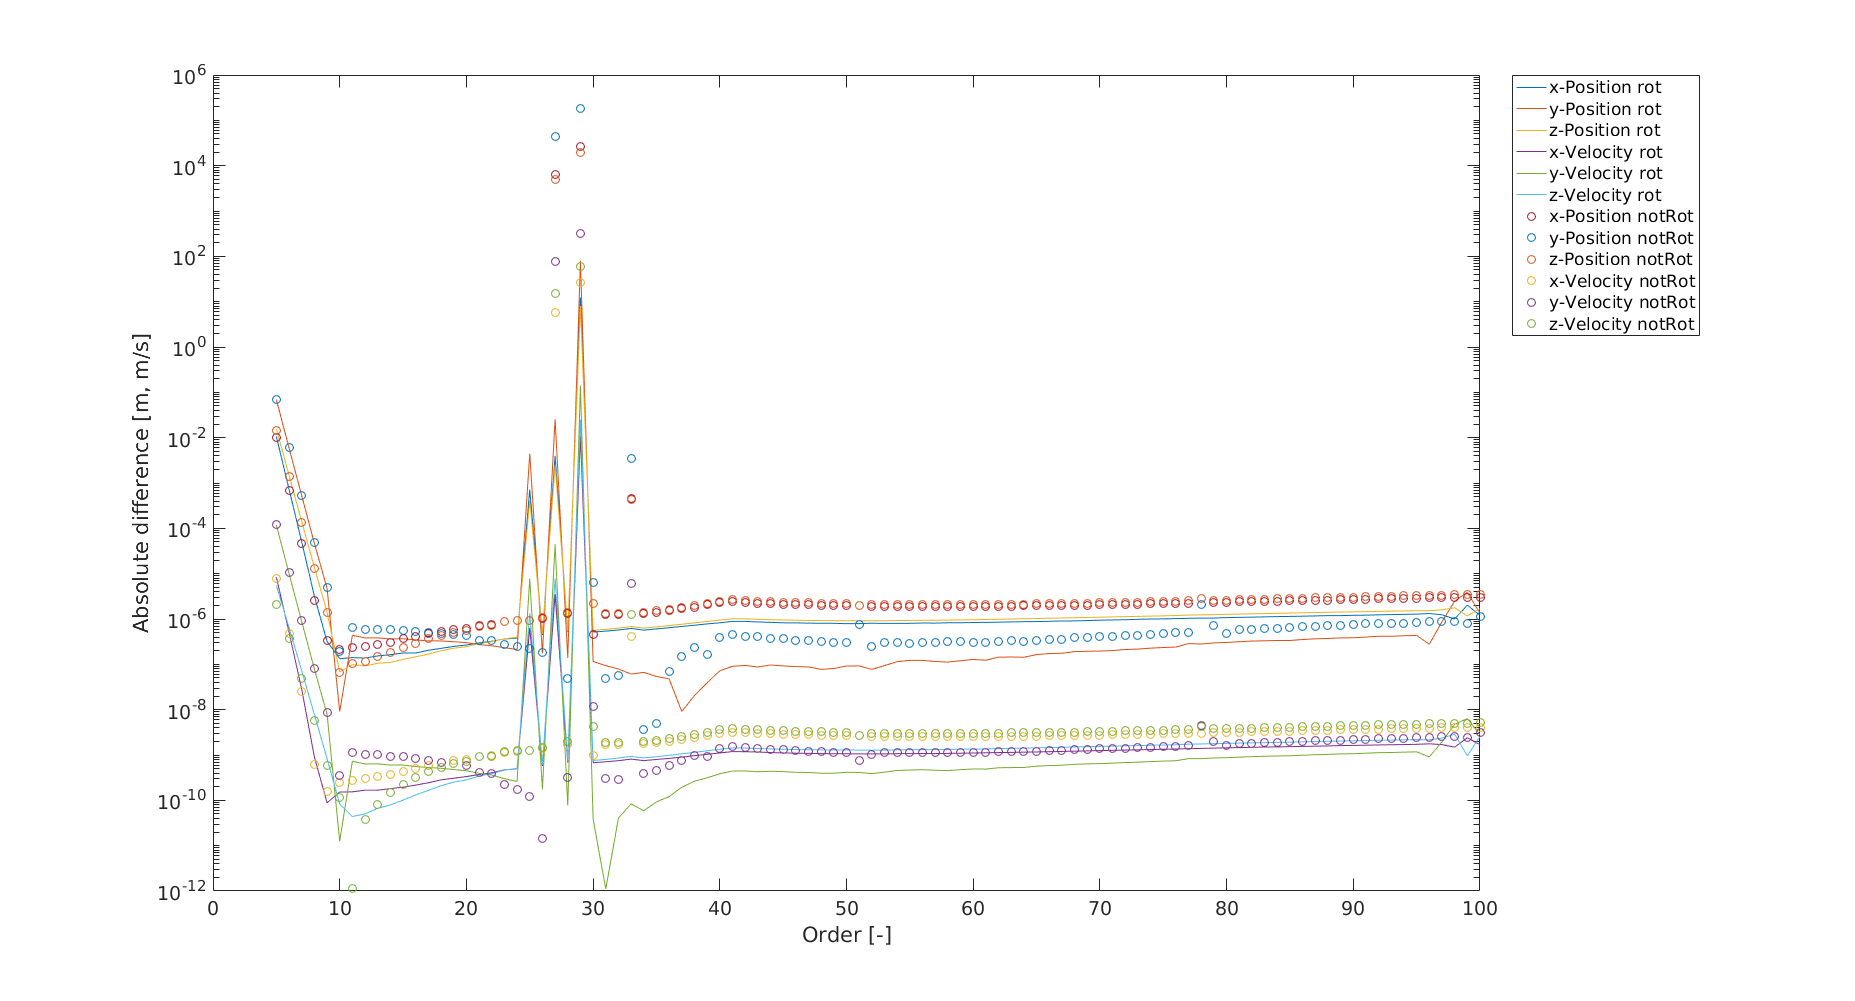
\includegraphics[width=1.1\textwidth]{figures/results/Order/orderVsRKFAbsoluteDifferenceCase1combined.png}\label{subfig:orderVsRKFAbsoluteDifferenceCase1combined}}\\
 
 
\subfloat[]{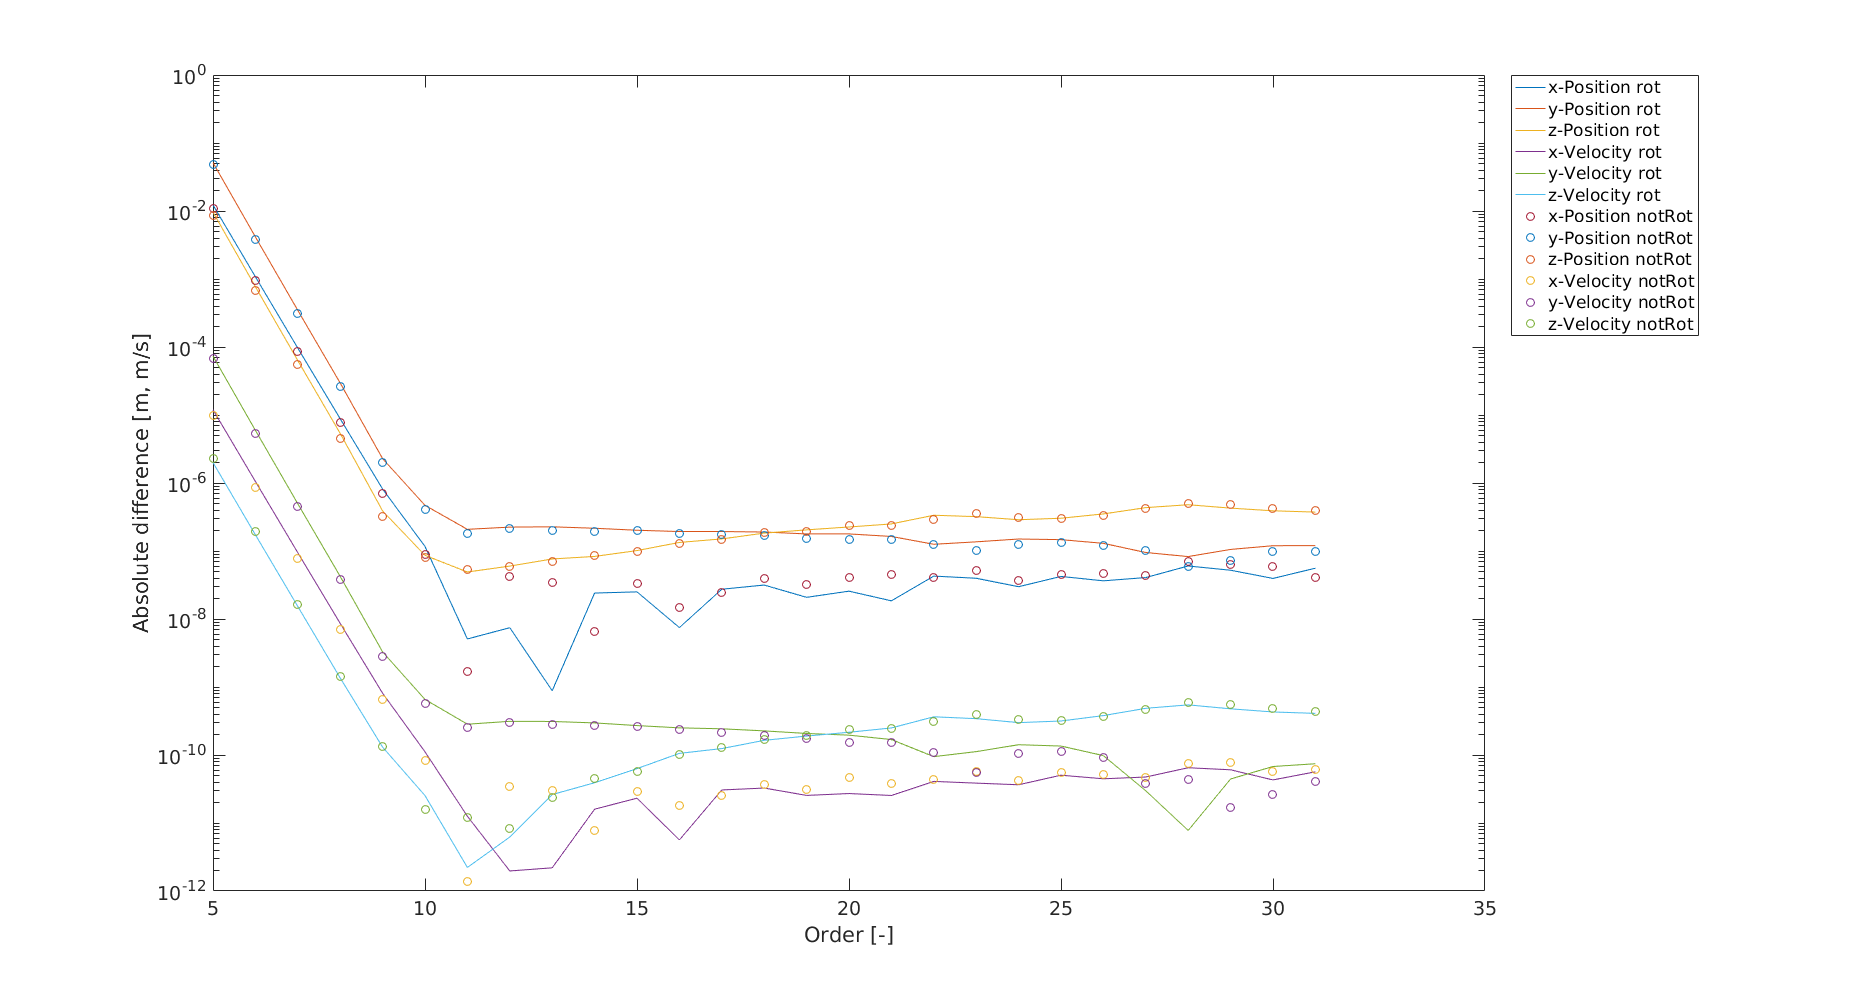
\includegraphics[width=1.1\textwidth]{figures/results/Order/orderVsRKFAbsoluteDifferenceCase2combined.png}\label{subfig:orderVsRKFAbsoluteDifferenceCase2combined}}
\caption{Difference with respect to \ac{RKF} case for rotating and non-rotating Mars \protect\subref{subfig:orderVsRKFAbsoluteDifferenceCase1combined} case 1,  \protect\subref{subfig:orderVsRKFAbsoluteDifferenceCase2combined} case 2 } 
\label{fig:orderVsRKFAbsoluteDifferenceCase1combined} 
\end{figure}


\section{Error tolerance}
\label{sec:errorTolerance}
The error tolerance is used to determine the required step-size during the integration. A high error tolerance (say 10$^{-5}$) will therefore provide an end result that is less accurate than a lower error tolerance (such as 10$^{-15}$). For the \ac{RKF78} provided by \ac{Tudat} the lowest accuracy that can be used is 10$^{-15}$, which is why that accuracy is used as the nominal accuracy. When a range of error tolerances is examined the accuracy of the end state and the speed of convergence can be determined. The speed of convergence follows from the consecutive differences between the end states and the accuracy of the end states comes from the comparison to the nominal case. Both these characteristics will be examined and compared for \ac{RKF} and \ac{TSI}, see \Cref{subsec:errorToleranceCompRKF}, and for the rotating and non-rotating Mars described in \Cref{subsec:errorToleranceCompNotRot}. The cut-off criteria for case 1 was 789 seconds and 876 seconds for case 2 and both cases were run without live data collection.


%Mention what I want to discuss in this section.


\subsection{Comparison with \ac{RKF78}}
\label{subsec:errorToleranceCompRKF}
The speed of convergence is important because it shows the relationship between the different error tolerances. If the differences are small it means that the change in error tolerance had a small effect. If the consecutive difference is large, it means that the solution has not yet converged. \Cref{fig:errorToleranceVsConsecutiveDifferenceCase1RKFTSIpositionSmall} shows the consecutive differences in position and velocity for the two cases for both integration methods. Here it can clearly be seen that \ac{TSI} converges much faster than \ac{RKF}. The curve of \ac{RKF} lies quite a bit higher, which means that the differences are larger, and thus it converges slower than \ac{TSI}.


%Show the faster convergence of end state before circularisation.


%Graphs needed:
%
%- Consecutive difference graphs RKF and TSI combined for case 1 \\
%- Consecutive difference graphs RKF and TSI combined for case 2 \\
%- Nominal case difference in end state before circularisation RKF and TSI combined case 1 \\
%- Nominal case difference in end state before circularisation RKF and TSI combined case 2 \\

\begin{figure}[H]
\centering
\subfloat[]{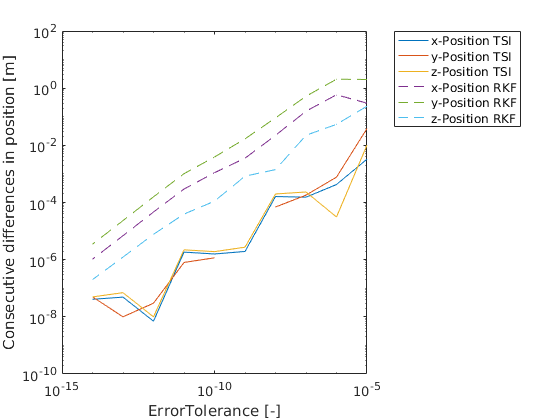
\includegraphics[width=3.1in]{figures/results/errorTolerance/errorToleranceVsConsecutiveDifferenceCase1RKFTSIpositionSmall.png}\label{subfig:errorToleranceVsConsecutiveDifferenceCase1RKFTSIpositionSmall}} 
\subfloat[]{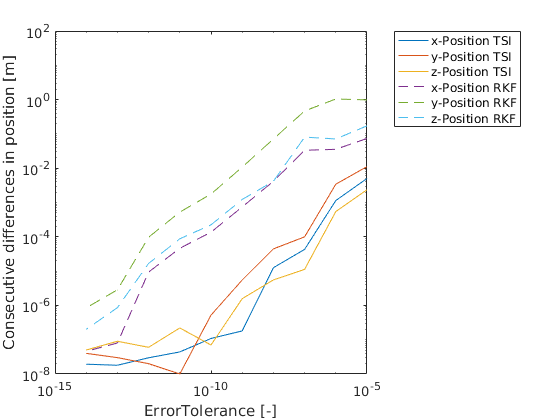
\includegraphics[width=3.1in]{figures/results/errorTolerance/errorToleranceVsConsecutiveDifferenceCase2RKFTSIpositionSmall.png} \label{subfig:errorToleranceVsConsecutiveDifferenceCase2RKFTSIpositionSmall}}\\
 
\subfloat[]{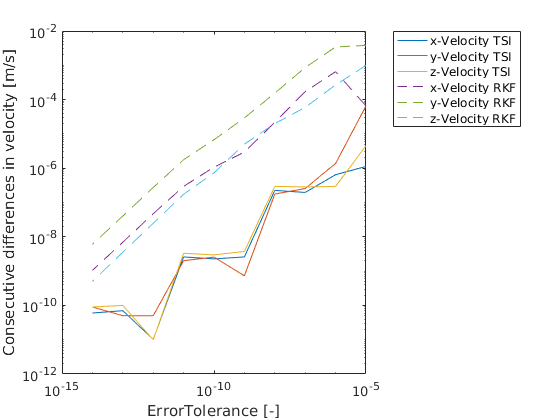
\includegraphics[width=3.1in]{figures/results/errorTolerance/errorToleranceVsConsecutiveDifferenceCase1RKFTSIvelocitySmall.png}\label{subfig:errorToleranceVsConsecutiveDifferenceCase1RKFTSIvelocitySmall}} 
\subfloat[]{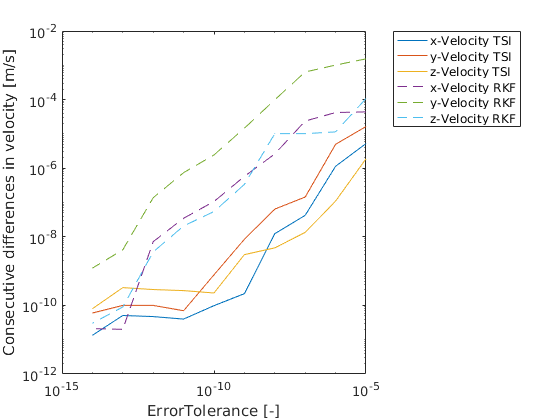
\includegraphics[width=3.1in]{figures/results/errorTolerance/errorToleranceVsConsecutiveDifferenceCase2RKFTSIvelocitySmall.png}\label{subfig:errorToleranceVsConsecutiveDifferenceCase2RKFTSIvelocitySmall}}
\caption{Error tolerance versus consecutive difference between end states before circularisation for \ac{TSI} and \ac{RKF} \protect\subref{subfig:errorToleranceVsConsecutiveDifferenceCase1RKFTSIpositionSmall} case 1 position, \protect\subref{subfig:errorToleranceVsConsecutiveDifferenceCase2RKFTSIpositionSmall} case 2 position, \protect\subref{subfig:errorToleranceVsConsecutiveDifferenceCase1RKFTSIvelocitySmall} case 1 velocity, \protect\subref{subfig:errorToleranceVsConsecutiveDifferenceCase2RKFTSIvelocitySmall} case 2 velocity } 
\label{fig:errorToleranceVsConsecutiveDifferenceCase1RKFTSIpositionSmall} 
\end{figure} 

A similar comparison can be done when comparing each of the end states directly to the nominal end state. The result is a nominal absolute difference graph as presented in \Cref{fig:errorToleranceVsNominalAbsoluteDifferenceCase1RKFTSIpositionSmall} for position and velocity and both cases. Here it can be seen that the accuracy of the position at an error tolerance of 10$^{-5}$ is already in cm for \ac{TSI} whereas this accuracy is only reached at an error tolerance of 10$^{-9}$ for \ac{RKF}. For the velocity the \ac{TSI} accuracy is in the order of 10 $\mu$m at this initial error tolerance which also is reached at an error tolerance of 10$^{-9}$ using \ac{TSI}. This means that \ac{TSI} is, on average, more accurate at any given error tolerance.  

\begin{figure}[H]
\centering
\subfloat[]{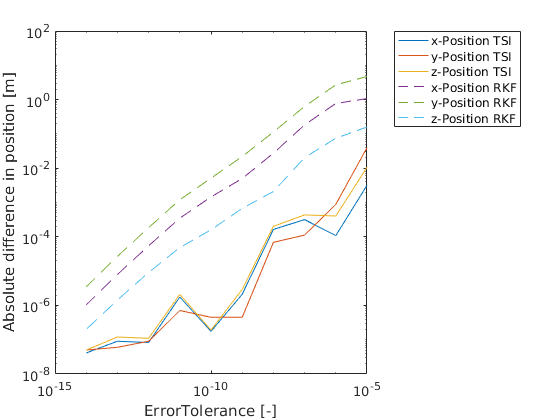
\includegraphics[width=3.1in]{figures/results/errorTolerance/errorToleranceVsNominalAbsoluteDifferenceCase1RKFTSIpositionSmall.png}\label{subfig:errorToleranceVsNominalAbsoluteDifferenceCase1RKFTSIpositionSmall}} 
\subfloat[]{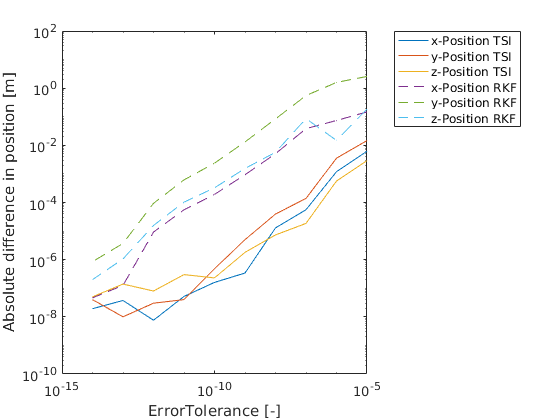
\includegraphics[width=3.1in]{figures/results/errorTolerance/errorToleranceVsNominalAbsoluteDifferenceCase2RKFTSIpositionSmall.png} \label{subfig:errorToleranceVsNominalAbsoluteDifferenceCase2RKFTSIpositionSmall}}\\
 
\subfloat[]{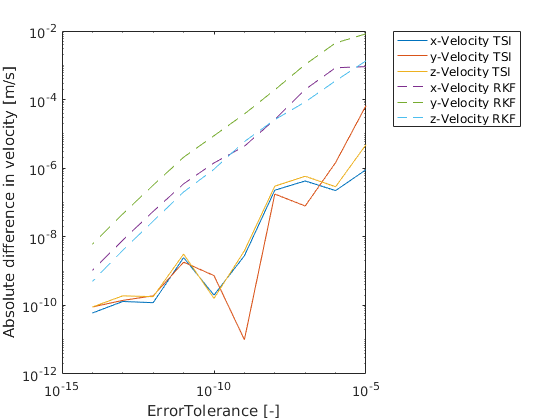
\includegraphics[width=3.1in]{figures/results/errorTolerance/errorToleranceVsNominalAbsoluteDifferenceCase1RKFTSIvelocitySmall.png}\label{subfig:errorToleranceVsNominalAbsoluteDifferenceCase1RKFTSIvelocitySmall}} 
\subfloat[]{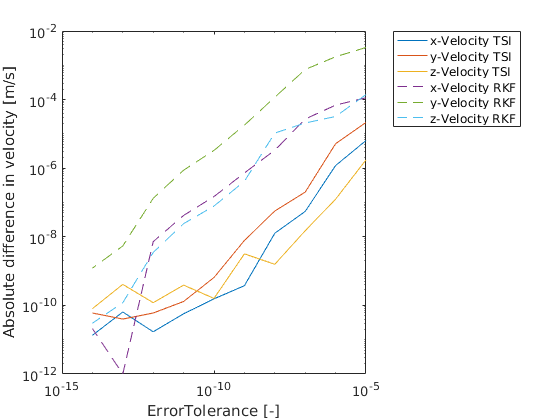
\includegraphics[width=3.1in]{figures/results/errorTolerance/errorToleranceVsNominalAbsoluteDifferenceCase2RKFTSIvelocitySmall.png}\label{subfig:errorToleranceVsNominalAbsoluteDifferenceCase2RKFTSIvelocitySmall}}
\caption{Error tolerance versus nominal absolute difference between end states before circularisation for \ac{TSI} and \ac{RKF} \protect\subref{subfig:errorToleranceVsNominalAbsoluteDifferenceCase1RKFTSIpositionSmall} case 1 position, \protect\subref{subfig:errorToleranceVsNominalAbsoluteDifferenceCase2RKFTSIpositionSmall} case 2 position, \protect\subref{subfig:errorToleranceVsNominalAbsoluteDifferenceCase1RKFTSIvelocitySmall} case 1 velocity, \protect\subref{subfig:errorToleranceVsNominalAbsoluteDifferenceCase2RKFTSIvelocitySmall} case 2 velocity } 
\label{fig:errorToleranceVsNominalAbsoluteDifferenceCase1RKFTSIpositionSmall} 
\end{figure} 

Another important observation can be made when looking at the difference in function evaluations and CPU time for each error tolerance for both \ac{RKF} and \ac{TSI}. The values for both cases are shown in \Cref{tab:RKFvsTSIfunctionEvaluationAndCPUtime}.



\begin{table}[H]
\begin{center}
\caption{Number of function evaluations and CPU time for \ac{RKF} and \ac{TSI}}
\label{tab:RKFvsTSIfunctionEvaluationAndCPUtime}
\begin{tabular}{|l|p{1.5cm}|p{1.5cm}|l|l|p{1.5cm}|p{1.5cm}|l|l|}
\hline 
\textbf{Error}  & \multicolumn{4}{c|}{\textbf{Case 1}} & \multicolumn{4}{c|}{\textbf{Case 2}} \\ \cline{2-9}

\textbf{tolerance} & \multicolumn{2}{c|}{Number of evaluations} & \multicolumn{2}{c|}{CPU time [ms]}& \multicolumn{2}{c|}{Number of evaluations} & \multicolumn{2}{c|}{CPU time [ms]} \\ \cline{2-9}

& \textbf{\ac{RKF}} &
\textbf{\ac{TSI}} & \textbf{\ac{RKF}} & \textbf{\ac{TSI}} & \textbf{\ac{RKF}} &
\textbf{\ac{TSI}} & \textbf{\ac{RKF}} & \textbf{\ac{TSI}} \\ \hline \hline

10$^{-5}$ & 169 & 24 & 0.419 &4.703 &156 &24 &0.392 &5.353 \\ \hline
10$^{-6}$ & 182 & 24 & 0.432 &4.57 &182 &25 &0.49 &5.518 \\ \hline
10$^{-7}$ & 221 & 26 & 0.542 &4.769 &208 &27 &0.527 &5.823 \\ \hline
10$^{-8}$ & 260 & 29 & 0.614 &5.272 &247 &29 &0.567 &6.354 \\ \hline
10$^{-9}$ & 312 & 30 & 0.823 &5.571 &286 &30 &0.709 &6.439 \\ \hline
10$^{-10}$ & 364 & 32 & 0.845 &5.685 &338 &33 &0.789 &7.083 \\ \hline
10$^{-11}$ & 455 & 36 & 1.032 &6.227 &390 &36 &0.904 &7.454 \\ \hline
10$^{-12}$ & 546 & 38 & 1.277 &6.506 &546 &39 &1.231 &8.02 \\ \hline
10$^{-13}$ & 702 & 41 & 1.541 &7.062 &728 &41 &1.604 &8.627 \\ \hline
10$^{-14}$ & 910 & 42 & 1.965 &7.227 &936 &45 &2.055 &9.538 \\ \hline
10$^{-15}$ & 1222 & 46 & 2.666 &7.754 &1300 &47 &2.851 &9.538 \\ \hline


\end{tabular}
\end{center}
\end{table}

Here one evaluation is defined as running through the derivative equations once. For \ac{TSI} this means that each time step, one evaluation is performed because all desired derivatives are computed during one computational run. In the case of \ac{RKF78} however, each time step consists of 13 computational runs. \Cref{tab:RKFvsTSIfunctionEvaluationAndCPUtime} shows that for both cases the number of evaluations of \ac{RKF} are approximately one order more at the high error tolerances but almost two orders higher at the lowest tolerance compared to \ac{TSI}. This means that a decrease in error tolerance results in a large increase in number of evaluations for \ac{RKF} but a relatively small increase for \ac{TSI}. For both cases, the number of evaluations is not even doubled from the highest to the lowest tolerance, whereas the maximum number of evaluations for \ac{RKF} is 7 to 8 times more. \\

This advantage however does not translate well to the CPU time where it can be seen that for most of the error tolerances \ac{RKF} is an order faster than \ac{TSI}. The similar increase in CPU time for both integrators is nevertheless still observed. An explanation for the large difference in CPU time could be that \ac{TSI} was not optimally programmed and thus results in a relatively high CPU time. Further analysis is required.

%Compare the number of function evaluations and explain why you should look at the function evaluations in such a manner. So explain that RKF does 13 function evaluations per step and TSI only does one.

%Tables needed:
%
%- Either accuracy of separate coordinates or simply radius in metres \\
%- Either accuracy of separate velocities or simply ground velocity in metres/second \\


\subsection{Comparison with non-rotating Mars}
\label{subsec:errorToleranceCompNotRot}
Looking at the rotating Mars and non-rotating Mars runs, a noticeable difference in the CPU time can be observed as shown in \Cref{fig:orderVsCPUcase1combined}. In both cases the non-rotating Mars run is approximately 0.2 ms faster. This is similar to what was observed with the order runs.


%Compare the rotating case with the non-rotating case and see if the convergence speed is different. 

%Graphs needed: 
%
%- CPU time vs error tolerance case 1 combined \\
%- CPU time vs error tolerance case 2 combined \\
%- Consecutive difference in end state before circularisation combined for case 1 \\
%- Consecutive difference in end state before circularisation combined for case 2 \\
%- Nominal case difference in end state before circularisation combined for case 1 \\
%- Nominal case difference in end state before circularisation combined for case 2 \\

\begin{figure}[H]
\centering
\subfloat[]{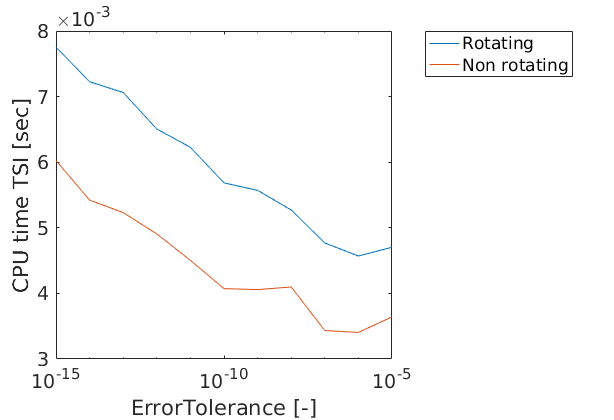
\includegraphics[scale=0.5]{figures/results/errorTolerance/errorToleranceVsCPUcase1combined.png}\label{subfig:errorToleranceVsCPUcase1combined}} 
\subfloat[]{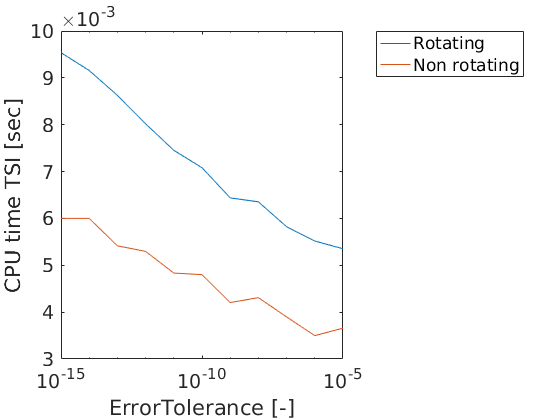
\includegraphics[scale=0.5]{figures/results/errorTolerance/errorToleranceVsCPUcase2combined.png}\label{subfig:errorToleranceVsCPUcase2combined}}
\caption{Error tolerance versus CPU time for rotating and non-rotating Mars \protect\subref{subfig:errorToleranceVsCPUcase1combined} case 1,  \protect\subref{subfig:errorToleranceVsCPUcase2combined} case 2 } 
\label{fig:orderVsCPUcase1combined} 
\end{figure} 

The real question is, is there a noticeable difference in the convergence speed and the accuracy? This question can be answered by looking at \Cref{fig:errorToleranceVsConsecutiveDifferenceCase1combinedSmall,fig:errorToleranceVsNominalAbsoluteDifferenceCase1combinedSmall}.
Here it can be seen that the rotation of Mars does not have a significant influence on the convergence speed nor the accuracy of the results.

\begin{figure}[H]
\centering
\subfloat[]{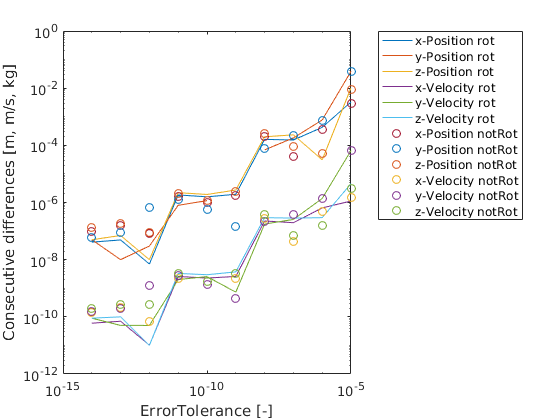
\includegraphics[width=3.1in]{figures/results/errorTolerance/errorToleranceVsConsecutiveDifferenceCase1combinedSmall.png}\label{subfig:errorToleranceVsConsecutiveDifferenceCase1combinedSmall}} 
\subfloat[]{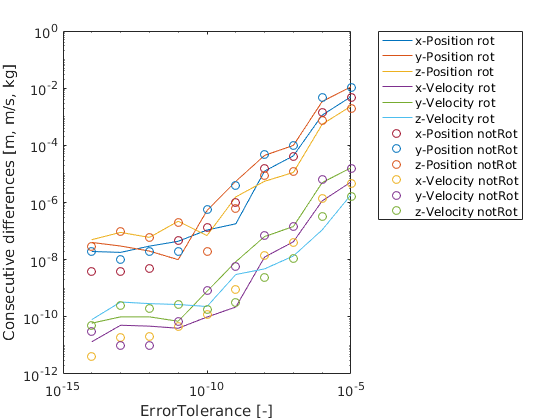
\includegraphics[width=3.1in]{figures/results/errorTolerance/errorToleranceVsConsecutiveDifferenceCase2combinedSmall.png}\label{subfig:errorToleranceVsConsecutiveDifferenceCase2combinedSmall}}
\caption{Error tolerance versus consecutive difference for rotating and non-rotating Mars \protect\subref{subfig:errorToleranceVsConsecutiveDifferenceCase1combinedSmall} case 1,  \protect\subref{subfig:errorToleranceVsConsecutiveDifferenceCase2combinedSmall} case 2 } 
\label{fig:errorToleranceVsConsecutiveDifferenceCase1combinedSmall} 
\end{figure} 

\begin{figure}[H]
\centering
\subfloat[]{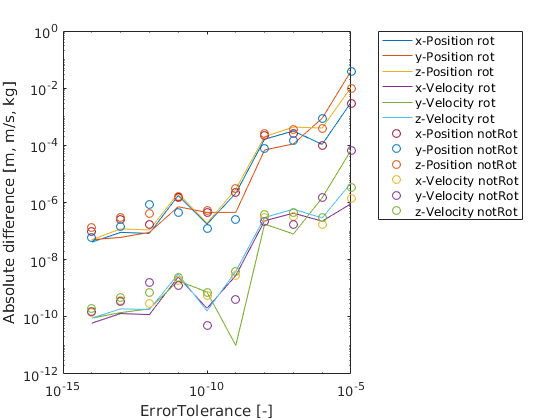
\includegraphics[width=3.1in]{figures/results/errorTolerance/errorToleranceVsNominalAbsoluteDifferenceCase1combinedSmall.png}\label{subfig:errorToleranceVsNominalAbsoluteDifferenceCase1combinedSmall}} 
\subfloat[]{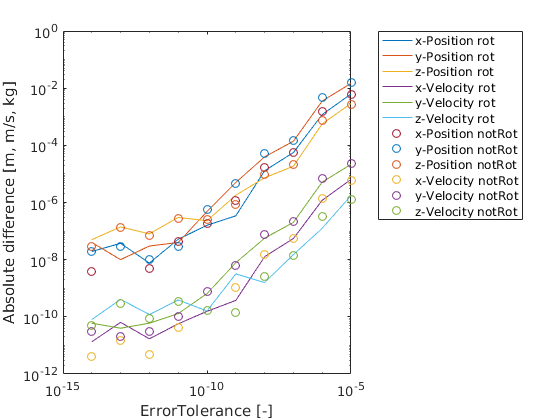
\includegraphics[width=3.1in]{figures/results/errorTolerance/errorToleranceVsNominalAbsoluteDifferenceCase2combinedSmall.png}\label{subfig:errorToleranceVsNominalAbsoluteDifferenceCase2combinedSmall}}
\caption{Error tolerance versus nominal absolute difference for rotating and non-rotating Mars \protect\subref{subfig:errorToleranceVsNominalAbsoluteDifferenceCase1combinedSmall} case 1,  \protect\subref{subfig:errorToleranceVsNominalAbsoluteDifferenceCase2combinedSmall} case 2 } 
\label{fig:errorToleranceVsNominalAbsoluteDifferenceCase1combinedSmall} 
\end{figure} 


%Tables needed:
%
%- Either accuracy of separate coordinates or simply radius in metres \\
%- Either accuracy of separate velocities or simply ground velocity in metres/second \\


\section{Multiple runs}
\label{sec:multipleRuns}
In \Cref{subsec:errorToleranceCompNotRot} it was shown that in this thesis research, the \ac{TSI} turned out to be slower than \ac{RKF} for both tested cases. This in contrary to the reference research. Therefore it is a good idea to look at the differences that could occur when measuring CPU time for different runs. In this section the nominal case has been run 5000 times in sequence for both \ac{RKF} and \ac{TSI} (\Cref{subsec:timeCompRKF}) using a rotating and a non-rotating Mars (\Cref{subsec:timeCompNotRot}). If the computer and the CPU measurements would be perfect, there should be no difference in CPU time and there would simply be two lines. This, interestingly enough, is not the case.\\

\noindent
The graphs shown in this section can also be found enlarged in \Cref{app:appendixG-Results}.

\subsection{Comparison with \ac{RKF78}}
\label{subsec:timeCompRKF}
Again the notion that \ac{RKF} is faster than \ac{TSI} is confirmed when looking at \Cref{fig:multiRunVsCPUcase1RKFTSIsmall}, however for both cases there is not one single line per integrator. Instead several outliers and patterns can be observed. 

%Show that RKF is faster than TSI at the moment. Explain why this might be the case and why this was unexpected. 
%
%Also explain the outliers and different patterns visible. 
%
%Graphs needed:
%
%- Combined RKF and TSI 5000 run plot for case 1 \\
%- Combined RKF and TSI 5000 run plot for case 2 \\

\begin{figure}[H]
\centering
\subfloat[]{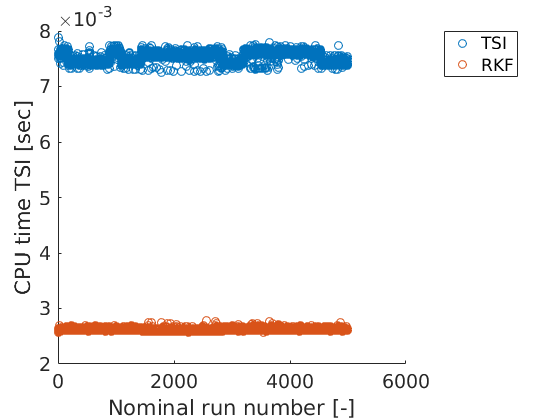
\includegraphics[width=3.1in]{figures/results/multiRun/multiRunVsCPUcase1RKFTSIsmall.png}\label{subfig:multiRunVsCPUcase1RKFTSIsmall}} 
\subfloat[]{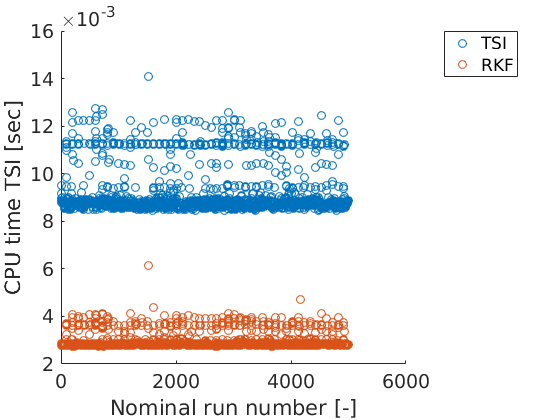
\includegraphics[width=3.1in]{figures/results/multiRun/multiRunVsCPUcase2RKFTSIsmall.png}\label{subfig:multiRunVsCPUcase2RKFTSIsmall}}
\caption{Nominal runs versus CPU time comparison between \ac{RKF} and \ac{TSI} \protect\subref{subfig:multiRunVsCPUcase1RKFTSIsmall} case 1,  \protect\subref{subfig:multiRunVsCPUcase2RKFTSIsmall} case 2 } 
\label{fig:multiRunVsCPUcase1RKFTSIsmall} 
\end{figure} 

For case 1 it can be seen that there were some periods where the CPU time was slightly higher. This is even clearer for case 2 where two different CPU levels can be distinguished and many random CPU times in between. The CPU time is computed using the internal clock of the computer. And it could occur that background programs are run while the integration is running. In such a case, the CPU time computed for that particular integration run can turn out to be higher than expected because the internal clock cannot differentiate between the simulation program and all other programs running at that same instance. Therefore, even if the same nominal case is run, the CPU time could still be 30\% higher or more. 

%Table needed:
%
%- Lowest CPU time for both RKF and TSI \\



\subsection{Comparison with non-rotating Mars}
\label{subsec:timeCompNotRot}
The effect of a program running in the background during a simulation run becomes even more clear when looking at the rotating and non-rotating Mars CPU times shown in \Cref{fig:multiRunVsCPUcase1combinedSmall}. 


%Show the notable difference between the rotating and non-rotating case. Explain why this is the case.
%
%Graphs needed:
%
%- Combined 5000 run plot rot and not rot for case 1 \\
%- Combined 5000 run plot rot and not rot for case 2 \\


\begin{figure}[H]
\centering
\subfloat[]{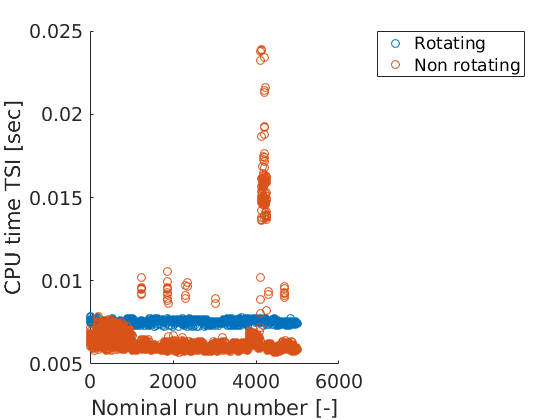
\includegraphics[width=3.1in]{figures/results/multiRun/multiRunVsCPUcase1combinedSmall.png}\label{subfig:multiRunVsCPUcase1combinedSmall}} 
\subfloat[]{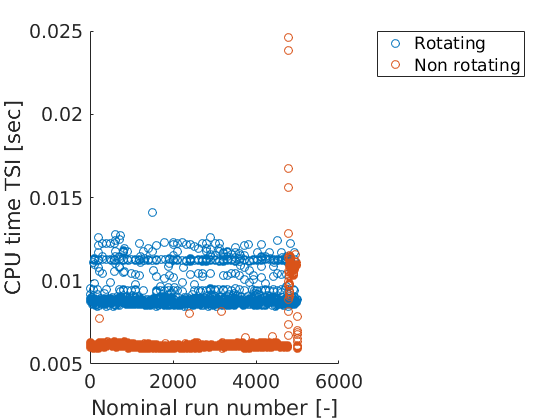
\includegraphics[width=3.1in]{figures/results/multiRun/multiRunVsCPUcase2combinedSmall.png}\label{subfig:multiRunVsCPUcase2combinedSmall}}
\caption{Nominal runs versus CPU time for rotating and non-rotating Mars \protect\subref{subfig:multiRunVsCPUcase1combinedSmall} case 1,  \protect\subref{subfig:multiRunVsCPUcase2combinedSmall} case 2 } 
\label{fig:multiRunVsCPUcase1combinedSmall} 
\end{figure} 

Here it can be seen that, on average, the non-rotating Mars runs are fasters than the rotating Mars runs, which is similar to what has been observed before. However, in both cases there was a spike where the CPU time suddenly increased tremendously for the non-rotating runs. This shows, that at that time a program (or process) was running in the background and clearly affected the performance of the simulation a lot. This means that CPU time is not always an accurate representation of the performance of the simulation. As a matter of fact, if the same program would be run on a different computer, the CPU times could be completely different. But it would still show the same relationship between the rotating and non-rotating Mars runs as well as \ac{RKF} and \ac{TSI} and does therefore not explain why \ac{TSI} is so much slower compared to \ac{RKF}.




\section{Launch altitude}
\label{sec:launchAltitude}
From now on only the rotating runs and the non-rotating runs will be compared. This can be done because \ac{TSI} has proven to be accurate compared to \ac{RKF} producing similar results. Thus it is only interesting to look at the effect of the different parameters on the performance of \ac{TSI}. In this case the effect on CPU time, consecutive difference and absolute difference will be investigated as well as effect on end radius and end velocity before cirularisation. Here the cut-off criteria for case 1 was an end time of 789 seconds and 856 seconds for case 2.\\

\noindent
In \Cref{fig:launchAltitudeVsCPUcase1combined} the launch altitude is plotted against the CPU time. This has been done for the altitude range from the candidate altitude of -0.6 km \ac{MOLA} to the maximum altitude where the \ac{MAV} could be launched from; 0.5 km \ac{MOLA}. In this case, no clear pattern can be observed due to the large differences in CPU time. Therefore it can be concluded that the launch altitude in this particular range does not have an effect on the CPU time.

%
%Only comparison with non-rotating Mars and simply look at the different altitudes and the effects
%
%Graphs needed:
%
%- CPU time vs order case 1 combined \\
%- CPU time vs order case 2 combined \\
%- Circularisation propellant mass comb case 1 (if different end conditions were used then once with comb and once just the case 1) \\
%- Circularisation propellant mass comb case 2 (if different end conditions were used then once with comb and once just the case 2) \\
- Consecutive differences end state before circularisation comb case 1 \\
- Consecutive differences end state before circularisation comb case 2 \\
- Differences nominal case end state before circularisation comb case 1 \\
- Differences nominal case end state before circularisation comb case 2 \\



\begin{figure}[H]
\centering
\subfloat[]{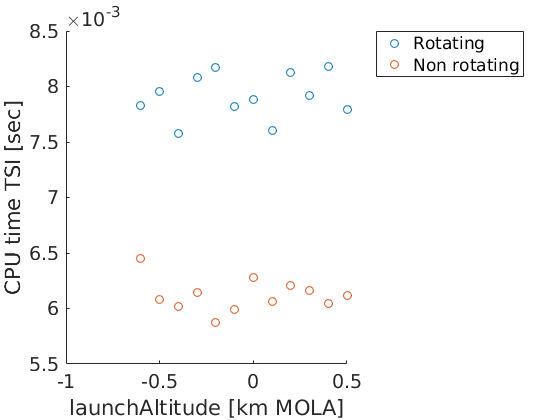
\includegraphics[width=3.1in]{figures/results/launchAltitude/launchAltitudeVsCPUcase1combined.png}\label{subfig:launchAltitudeVsCPUcase1combined}} 
\subfloat[]{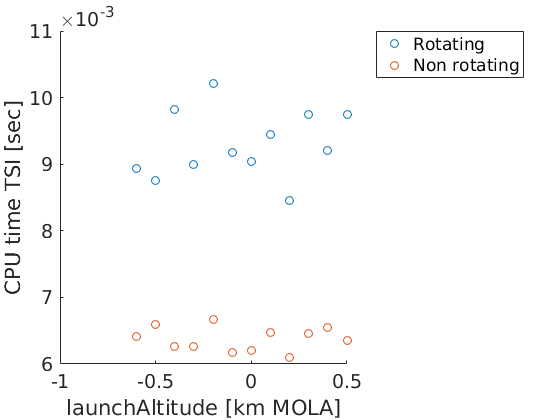
\includegraphics[width=3.1in]{figures/results/launchAltitude/launchAltitudeVsCPUcase2combined.png}\label{subfig:launchAltitudeVsCPUcase2combined}}
\caption{Launch altitude versus CPU time for rotating and non-rotating Mars \protect\subref{subfig:launchAltitudeVsCPUcase1combined} case 1,  \protect\subref{subfig:launchAltitudeVsCPUcase2combined} case 2 } 
\label{fig:launchAltitudeVsCPUcase1combined} 
\end{figure} 

\noindent
Randomness can also be observed when looking at the consecutive difference for the rotating runs in \Cref{fig:launchAltitudeVsConsecutiveDifferenceCase1combinedSmall}. Here the z-position and z-velocity show some slight deviations for case 1, and in the curves of case 2 the rotating states all show deviations. However, it is interesting to notice that no deviations are observed for the non-rotating runs, which means that all the deviations are caused by rotating effects. A similar behaviour can be observed in the nominal absolute difference graphs presented in \Cref{fig:launchAltitudeVsNominalAbsoluteDifferenceCase1combinedSmall}. Here case 1 shows almost no deviations except for the z-position and z-velocity. However, again large deviations can be observed for case 2. These deviations can be caused by the fact that for case 2 the \ac{MAV} is launched due East but quickly heads South therefore going against the rotation of Mars and creating variations that are not observed for the non-rotating Mars.

\begin{figure}[H]
\centering
\subfloat[]{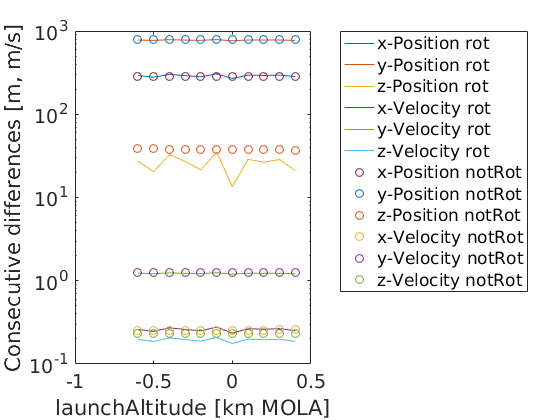
\includegraphics[width=3.1in]{figures/results/launchAltitude/launchAltitudeVsConsecutiveDifferenceCase1combinedSmall.png}\label{subfig:launchAltitudeVsConsecutiveDifferenceCase1combinedSmall}} 
\subfloat[]{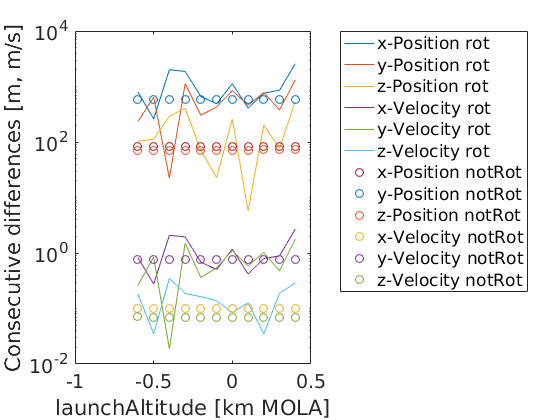
\includegraphics[width=3.1in]{figures/results/launchAltitude/launchAltitudeVsConsecutiveDifferenceCase2combinedSmall.png}\label{subfig:launchAltitudeVsConsecutiveDifferenceCase2combinedSmall}}
\caption{Launch altitude versus consecutive difference for rotating and non-rotating Mars \protect\subref{subfig:launchAltitudeVsConsecutiveDifferenceCase1combinedSmall} case 1,  \protect\subref{subfig:launchAltitudeVsConsecutiveDifferenceCase2combinedSmall} case 2 } 
\label{fig:launchAltitudeVsConsecutiveDifferenceCase1combinedSmall} 
\end{figure} 



\begin{figure}[H]
\centering
\subfloat[]{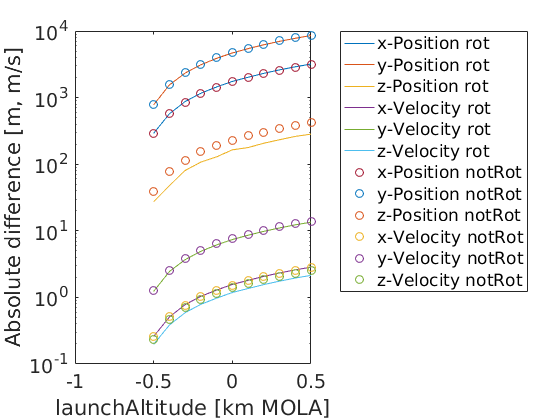
\includegraphics[width=3.1in]{figures/results/launchAltitude/launchAltitudeVsNominalAbsoluteDifferenceCase1combinedSmall.png}\label{subfig:launchAltitudeVsNominalAbsoluteDifferenceCase1combinedSmall}} 
\subfloat[]{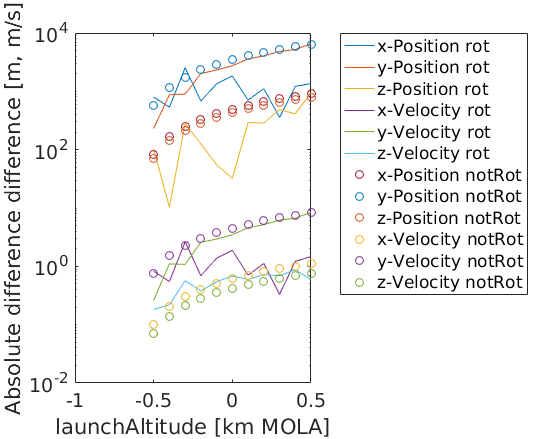
\includegraphics[width=3.1in]{figures/results/launchAltitude/launchAltitudeVsNominalAbsoluteDifferenceCase2combinedSmall.png}\label{subfig:launchAltitudeVsNominalAbsoluteDifferenceCase2combinedSmall}}
\caption{Launch altitude versus nominal absolute difference for rotating and non-rotating Mars \protect\subref{subfig:launchAltitudeVsNominalAbsoluteDifferenceCase1combinedSmall} case 1,  \protect\subref{subfig:launchAltitudeVsNominalAbsoluteDifferenceCase2combinedSmall} case 2 } 
\label{fig:launchAltitudeVsNominalAbsoluteDifferenceCase1combinedSmall} 
\end{figure} 

\noindent
Another example of the effect of the rotating Mars can be seen in the radius graphs in \Cref{fig:launchAltitudeVsRadiusCase1combined}. Because in both case 1 and 2 the \ac{MAV} is launched due East on the equator it is able to get an initial $\Delta$V boost. This increase in velocity compared to the non-rotating results in a final radius that is higher than the non-rotating Mars runs for both case 1 and case 2. It can also be observed that the radius of the final orbit increases with an increase in launch altitude. This could be a direct effect of both the drag and the gravitational acceleration, because the atmosphere becomes less dense and the gravitational acceleration becomes smaller the further away from the surface the \ac{MAV} is.



\begin{figure}[H]
\centering
\subfloat[]{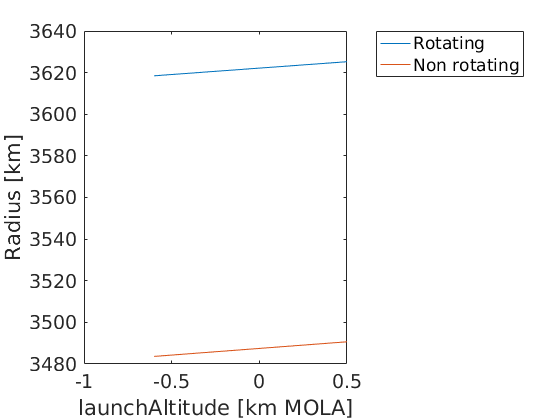
\includegraphics[width=3.1in]{figures/results/launchAltitude/launchAltitudeVsRadiusCase1combined.png}\label{subfig:launchAltitudeVsRadiusCase1combined}} 
\subfloat[]{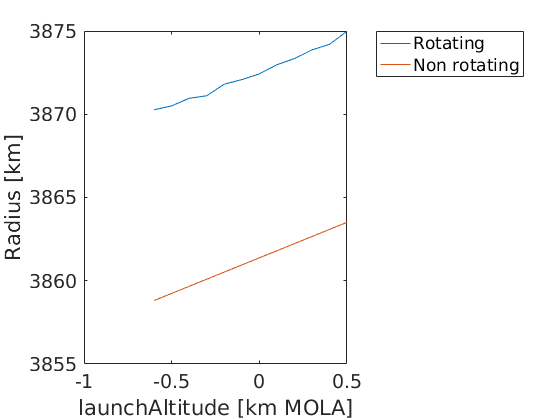
\includegraphics[width=3.1in]{figures/results/launchAltitude/launchAltitudeVsRadiusCase2combined.png}\label{subfig:launchAltitudeVsRadiusCase2combined}}
\caption{Launch altitude versus orbital radius for rotating and non-rotating Mars \protect\subref{subfig:launchAltitudeVsRadiusCase1combined} case 1,  \protect\subref{subfig:launchAltitudeVsRadiusCase2combined} case 2 } 
\label{fig:launchAltitudeVsRadiusCase1combined} 
\end{figure} 

\noindent 
In \Cref{fig:launchAltitudeVsRadiusCase1combined} the ground and inertial velocity for both cases and both rotating and non-rotating Mars have been plotted. These are the end velocities of the \ac{MAV} before circularisation. And because an increase in final radius was observed, a decrease in end velocity was expected and this is indeed observed for both cases. 


\begin{figure}[H]
\centering
\subfloat[]{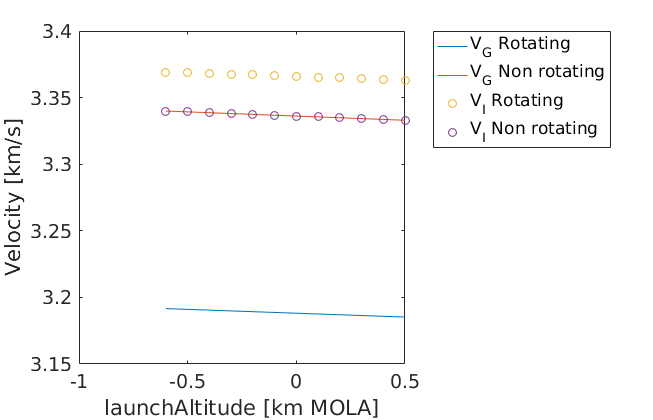
\includegraphics[scale=0.5]{figures/results/launchAltitude/launchAltitudeVsVelocityCase1combined.png}\label{subfig:launchAltitudeVsVelocityCase1combined}} 
\subfloat[]{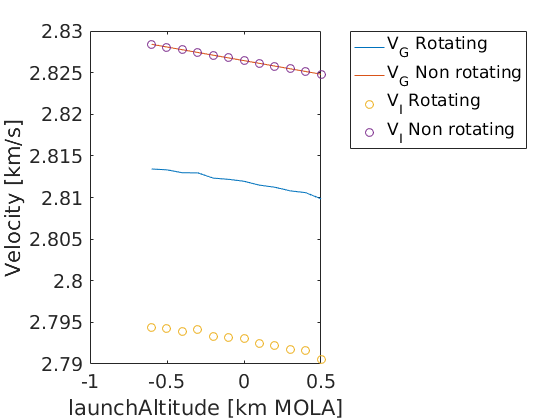
\includegraphics[scale=0.5]{figures/results/launchAltitude/launchAltitudeVsVelocityCase2combined.png}\label{subfig:launchAltitudeVsVelocityCase2combined}}
\caption{Launch altitude versus velocity for rotating and non-rotating Mars \protect\subref{subfig:launchAltitudeVsVelocityCase1combined} case 1,  \protect\subref{subfig:launchAltitudeVsVelocityCase2combined} case 2 } 
\label{fig:launchAltitudeVsVelocityCase1combined} 
\end{figure} 

\noindent
When comparing ground velocity it would be expected that the rotating Mars run would show a lower velocity because Mars is actually rotating with the \ac{MAV}. This effectively lowers the speed at which the \ac{MAV} travels as observed from the Martian surface. This is indeed seen in both cases. What is also noticeable is that there is fortunately no velocity difference between the inertial and ground velocity for the non-rotating case, which means that the rotation of Mars was indeed zero and the program is working properly. There is however a large difference between the ground and inertial velocity for the rotating runs, which is precisely the effective velocity boost from the rotating Mars.\\

\noindent
Finally it is interesting to notice the difference in end velocities between case 1 and case 2. Case 1 has an inertial velocity which is higher than the ground velocity and also the velocity for the non-rotating run. This is what one would expect for a \ac{MAV} that is launched due East. However, case 2 also launches due East and shows an inertial velocity for the rotating run which is lower than all other velocities. This can be explained by taking to account that these are all final velocities before the circularisation and remembering the trajectory profile of both cases as presented in \Cref{ch:verificationandvalidation}. The trajectory of case 1 takes the \ac{MAV} slightly North after launch, whereas in case 2 the trajectory goes South and even slightly West. This means that it is moving against the rotation of Mars and thus effectively loses some velocity when compared to both the ground velocity as well as the velocity in the non-rotating run. This effect was therefore expected.
More position and velocity graphs can be found in \Cref{app:appendixG-Results}.

%Tables needed:
%
%- Radius and difference with nominal case in m case 1 \\
%- Radius and difference with nominal case in m case 2 \\
%- Ground velocity and difference with nominal case in m case 1 \\
%- Ground velocity and difference with nominal case in m case 2 \\





\section{Launch latitude}
\label{sec:launchLatitude}
For the latitude comparisons, the CPU time, radius and velocity are compared. Additional graphs for the end states are provided in \Cref{app:appendixG-Results}. The cut-off criteria was an end time of 789 seconds for the first case and 783 seconds for the second case. Again starting with the CPU time as shown in \Cref{fig:launchLatitudeVsCPUcase1combined}. Even though the curves from case 1 and case 2 might look different, they show the same behaviour. Starting at the equator and ending on the North-pole, both graphs show that the CPU time of the rotating and the non-rotating case converge until they are practically the same on the North-pole. This clearly shows the effect of the rotating Mars on both cases, because this effect becomes smaller with an increase in latitude.



\begin{figure}[H]
\centering
\subfloat[]{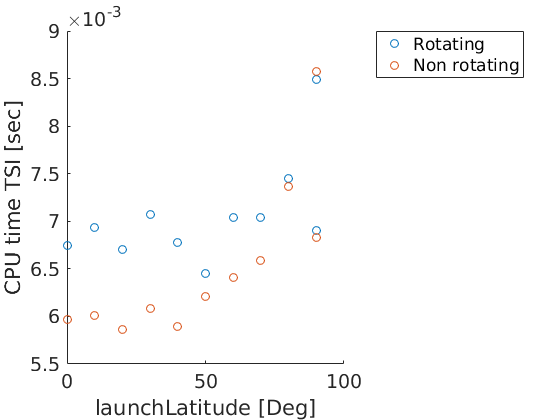
\includegraphics[width=3.1in]{figures/results/launchLatitude/launchLatitudeVsCPUcase1combined.png}\label{subfig:launchLatitudeVsCPUcase1combined}} 
\subfloat[]{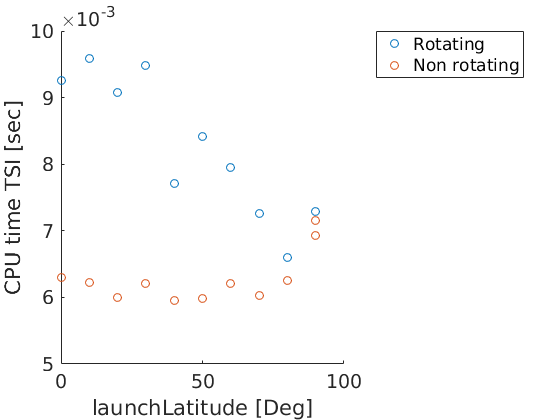
\includegraphics[width=3.1in]{figures/results/launchLatitude/launchLatitudeVsCPUcase2combined.png}\label{subfig:launchLatitudeVsCPUcase2combined}}
\caption{Launch latitude versus CPU time for rotating and non-rotating Mars \protect\subref{subfig:launchLatitudeVsCPUcase1combined} case 1,  \protect\subref{subfig:launchLatitudeVsCPUcase2combined} case 2 } 
\label{fig:launchLatitudeVsCPUcase1combined} 
\end{figure} 

\Cref{fig:launchLatitudeVsRadiusCase1combined} shows the radius for each of the launch latitudes for both cases. Again, as expected the launch latitude does not have an effect on the non-rotating runs, however it does seem to have a large effect on the rotating runs. 

\begin{figure}[H]
\centering
\subfloat[]{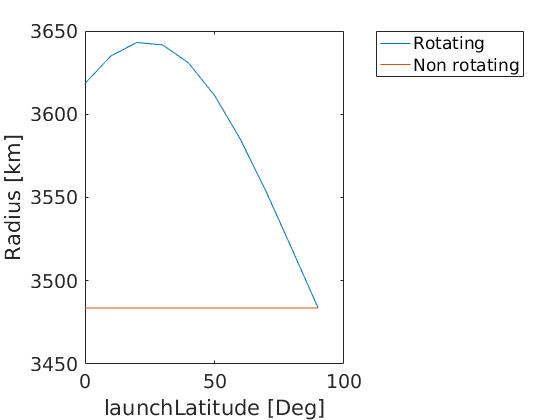
\includegraphics[width=3.1in]{figures/results/launchLatitude/launchLatitudeVsRadiusCase1combined.png}\label{subfig:launchLatitudeVsRadiusCase1combined}} 
\subfloat[]{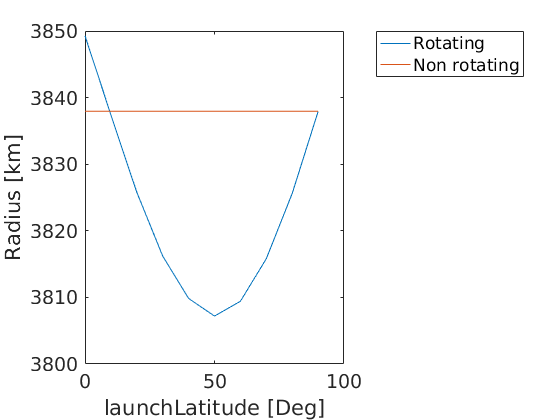
\includegraphics[width=3.1in]{figures/results/launchLatitude/launchLatitudeVsRadiusCase2combined.png}\label{subfig:launchLatitudeVsRadiusCase2combined}}
\caption{Launch latitude versus orbital radius for rotating and non-rotating Mars \protect\subref{subfig:launchLatitudeVsRadiusCase1combined} case 1,  \protect\subref{subfig:launchLatitudeVsRadiusCase2combined} case 2 } 
\label{fig:launchLatitudeVsRadiusCase1combined} 
\end{figure} 

\noindent
Looking at case 1, the end radius shows a sinusoidal effect with the highest end radius at 20 degrees. It is however interesting that case 2 shows an almost mirror effect, where the maximum end radius is reached using the nominal conditions, but still a sinusoidal behaviour can be identified. The minimum end radius is reached at 50 degrees and the non-rotating end radius is crossed at a launch latitude of approximately 10 degrees. This sinusoidal effect can only be attributed to the rotating effects which is similar for both case 1 and 2. They still look different though, which is due to the fact that both trajectories are very different. Case 1 launches due East and then North and case 2 launches due East and then South, South-West. Which means that the trajectories are practically mirrored, and this is also seen in the radius graphs. \\

\noindent
These effects are also shown in the velocity curves presented in \Cref{fig:launchLatitudeVsVelocityCase1combined}. Here the ground velocity shows the expected behaviour and a similar curve is also shown by the inertial velocity. However, for case 1 the inertial velocity starts above the non-rotating velocity and then drops below. This transition happens at the maximum radius, after which the curve follows slowly recovers to towards the non-rotating values. At that crossing point, the \ac{MAV} ends up due West, however this effect is maximum at a latitude of 50 degrees and becomes smaller again as soon as the latitude reaches the North-pole.

\begin{figure}[H]
\centering
\subfloat[]{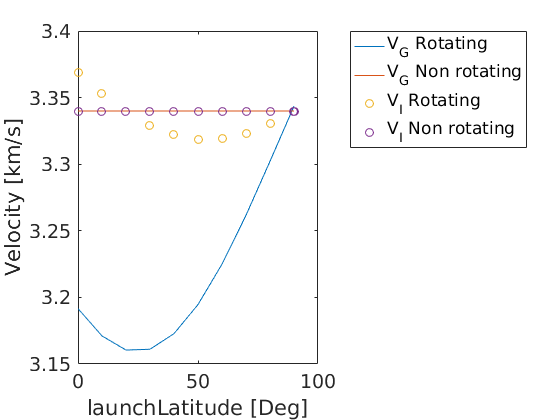
\includegraphics[width=3.1in]{figures/results/launchLatitude/launchLatitudeVsVelocityCase1combined.png}\label{subfig:launchLatitudeVsVelocityCase1combined}} 
\subfloat[]{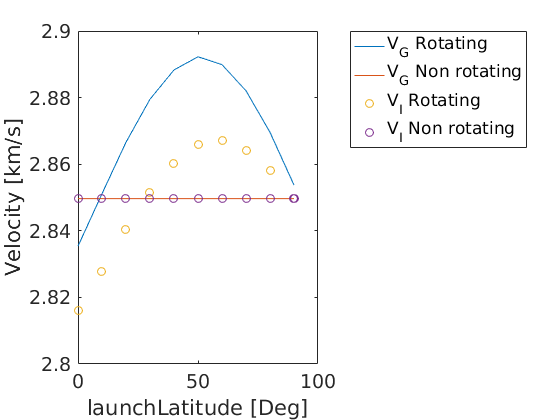
\includegraphics[width=3.1in]{figures/results/launchLatitude/launchLatitudeVsVelocityCase2combined.png}\label{subfig:launchLatitudeVsVelocityCase2combined}}
\caption{Launch latitude versus velocity for rotating and non-rotating Mars \protect\subref{subfig:launchLatitudeVsVelocityCase1combined} case 1,  \protect\subref{subfig:launchLatitudeVsVelocityCase2combined} case 2 } 
\label{fig:launchLatitudeVsVelocityCase1combined} 
\end{figure}



%Only comparison with non-rotating Mars and simply look at the different latitudes and the effects
%Show for both cases the differences in x,y and z position and velocity. Do case 1 and 2 look similar? Why do the graphs look a certain way?

%Graphs needed:
%
%%- CPU time vs order case 1 combined (if not random) \\
%%- CPU time vs order case 2 combined (if not random) \\
%- All position graphs case 1 \\ Appendix
%- All position graphs case 2 \\ Appendix
%- All velocity graphs case 1 \\ Appendix
%- All velocity graphs case 2 \\ Appendix

%- Circularisation propellant mass comb case 1 (if different end conditions were used then once with comb and once just the case 1) \\
%- Circularisation propellant mass comb case 2 (if different end conditions were used then once with comb and once just the case 2) \\
%- Consecutive differences end state before circularisation comb case 1 \\
%- Consecutive differences end state before circularisation comb case 2 \\
%- Differences nominal case end state before circularisation comb case 1 \\
%- Differences nominal case end state before circularisation comb case 2 \\


%Tables needed:
%
%- Radius and difference with nominal case in m case 1 \\
%- Radius and difference with nominal case in m case 2 \\
%- Ground velocity and difference with nominal case in m case 1 \\
%- Ground velocity and difference with nominal case in m case 2 \\
% 


\section{Launch longitude}
\label{sec:launchLongitude}
For the launch longitude, the cut-off criteria was an end time of 789 seconds for case 1 and 873 seconds for case 2. The longitude ($\tau$) has been varied from 0 to 330 degrees. Both the kinematic equations described in \Cref{eq:kinEqSp} and the dynamic equations described in \Cref{eq:dynEqSp} do not depend on the longitude. This means that no differences are expected between the different longitudes. \\

\noindent
In \Cref{fig:launchLongitudeVsCPUcase1combined} the launch longitude is plotted against the CPU time, and even though no two longitudes have the same CPU time there is still no significant difference, because the differences in CPU time can be explained by the arguments presented in \Cref{sec:multipleRuns}. 


%Only comparison with non-rotating Mars and simply look at the different longitudes and the effects
%Show for both cases the differences in x,y and z position and velocity. Do case 1 and 2 look similar? Why do the graphs look a certain way?
%
%Graphs needed:
%
%- CPU time vs order case 1 combined (if not random) \\
%- CPU time vs order case 2 combined (if not random) \\
%- All position graphs case 1 \\ Appendix
%- All position graphs case 2 \\ Appendix
%- All velocity graphs case 1 \\ Appendix
%- All velocity graphs case 2 \\ Appendix

%- Circularisation propellant mass comb case 1 (if different end conditions were used then once with comb and once just the case 1) \\
%- Circularisation propellant mass comb case 2 (if different end conditions were used then once with comb and once just the case 2) \\
%- Consecutive differences end state before circularisation comb case 1 \\
%- Consecutive differences end state before circularisation comb case 2 \\
%- Differences nominal case end state before circularisation comb case 1 \\
%- Differences nominal case end state before circularisation comb case 2 \\



\begin{figure}[H]
\centering
\subfloat[]{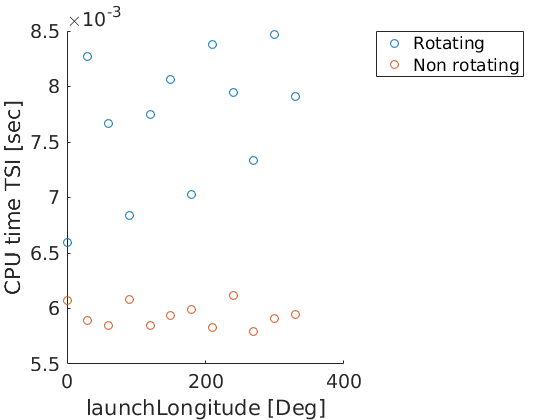
\includegraphics[width=3.1in]{figures/results/launchLongitude/launchLongitudeVsCPUcase1combined.png}\label{subfig:launchLongitudeVsCPUcase1combined}} 
\subfloat[]{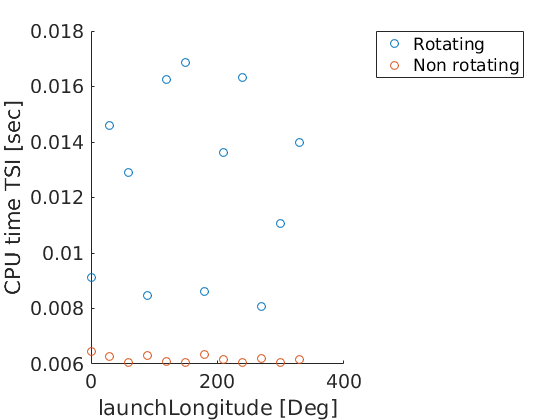
\includegraphics[width=3.1in]{figures/results/launchLongitude/launchLongitudeVsCPUcase2combined.png}\label{subfig:launchLongitudeVsCPUcase2combined}}
\caption{Launch longitude versus CPU time for rotating and non-rotating Mars \protect\subref{subfig:launchLongitudeVsCPUcase1combined} case 1,  \protect\subref{subfig:launchLongitudeVsCPUcase2combined} case 2 } 
\label{fig:launchLongitudeVsCPUcase1combined} 
\end{figure} 

\noindent
It is however more interesting to look at the differences in radius and velocity as shown in \Cref{fig:launchLongitudeVsRadiusCase1combined,fig:launchLongitudeVsVelocityCase1combined} respectively. Here it can be seen that for both the non-rotating as well as the rotating runs there are no noticeable differences for the end radius and end velocity of case 1. But case 2 does indeed show a difference in both graphs. As a matter of fact depending on the chosen launch longitude, the difference in end radius could be as large as 1 km (a more detailed graph with the differences between the non-rotating and rotating runs can be found in \Cref{app:appendixG-Results}, which show that case 1 also has a slight difference but at an order of metres). 


\begin{figure}[H]
\centering
\subfloat[]{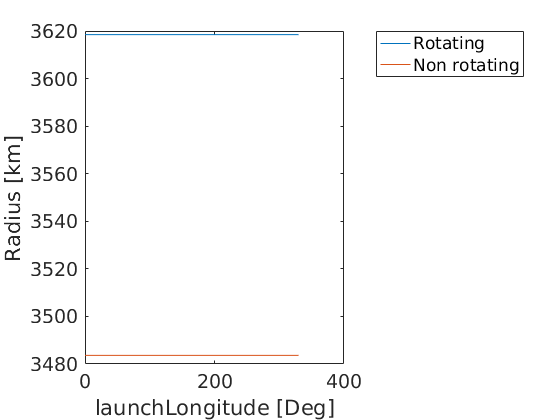
\includegraphics[width=3.1in]{figures/results/launchLongitude/launchLongitudeVsRadiusCase1combined.png}\label{subfig:launchLongitudeVsRadiusCase1combined}} 
\subfloat[]{\includegraphics[width=3.1in]{figures/results/launchLongitude/launchLongitudeVsRadiusCase2combined.png}\label{subfig:launchLongitudeVsRadiusCase2combined}}
\caption{Launch longitude versus orbital radius for rotating and non-rotating Mars \protect\subref{subfig:launchLongitudeVsRadiusCase1combined} case 1,  \protect\subref{subfig:launchLongitudeVsRadiusCase2combined} case 2 } 
\label{fig:launchLongitudeVsRadiusCase1combined} 
\end{figure} 

\begin{figure}[H]
\centering
\subfloat[]{\includegraphics[width=3.1in]{figures/results/launchLongitude/launchLongitudeVsVelocityCase1combined.png}\label{subfig:launchLongitudeVsVelocityCase1combined}} 
\subfloat[]{\includegraphics[width=3.1in]{figures/results/launchLongitude/launchLongitudeVsVelocityCase2combined.png}\label{subfig:launchLongitudeVsVelocityCase2combined}}
\caption{Launch longitude versus velocity for rotating and non-rotating Mars \protect\subref{subfig:launchLongitudeVsVelocityCase1combined} case 1,  \protect\subref{subfig:launchLongitudeVsVelocityCase2combined} case 2 } 
\label{fig:launchLongitudeVsVelocityCase1combined} 
\end{figure}

\noindent
The difference in end radius follows from a difference in velocity. Because the only difference between case 1 and case 2 is the input, these differences can be attributed to rounding errors.  It seems that different combinations of input values could create cases where the rounding errors can have a large effect. It is interesting to note that \ac{RKF} showed the same deviations.


\section{Flight-path angle}
\label{sec:flightPathAngle}
Previously, the cut-off criteria was always set to be a certain end time. However, for the \ac{FPA} it is better to set the cut-off criteria as the point when the simulation reaches the zero degree \ac{FPA}. This means that not only the final altitude will be different but also the simulation run time. It is expected that a \ac{MAV} launched at a lower launch \ac{FPA} will reach the cut-off criteria earlier compared to a high flight-path angle launch. A lower simulation time will equal fewer function evaluations. This is shown in \Cref{fig:FPAvsFunctionEvaluationsCase1combined}, where it is clear that for both the rotating and the non-rotating Mars runs the number of function evaluations decrease with a decrease in \ac{FPA} for both cases. It also shows that the number of function evaluations does not differ much compared to the non-rotating runs, but the two curves do seem to diverge slightly with higher \ac{FPA}. This is expected since the simulation run time is higher as well.  





%Only comparison with non-rotating Mars and simply look at the different Flight-path angles and the effects
%Show for both cases the differences in x,y and z position and velocity. Do case 1 and 2 look similar? Why do the graphs look a certain way?
%Explain why only a few runs could be done because of the huge initial effect that the FPA has because of the low velocity in the beginning.
%
%Graphs needed:

%- CPU time vs order case 1 combined (if not random) \\
%- CPU time vs order case 2 combined (if not random) \\
%- All position graphs case 1 \\
%- All position graphs case 2 \\
%- All velocity graphs case 1 \\
%- All velocity graphs case 2 \\

%- Circularisation propellant mass comb case 1 (if different end conditions were used then once with comb and once just the case 1) \\
%- Circularisation propellant mass comb case 2 (if different end conditions were used then once with comb and once just the case 2) \\
%- Consecutive differences end state before circularisation comb case 1 \\
%- Consecutive differences end state before circularisation comb case 2 \\
%- Differences nominal case end state before circularisation comb case 1 \\
%- Differences nominal case end state before circularisation comb case 2 \\


\begin{figure}[H]
\centering
\subfloat[]{\includegraphics[scale = 0.5]{figures/results/FPA/FPAvsFunctionEvaluationsCase1combined.png}\label{subfig:FPAvsFunctionEvaluationsCase1combined}} 
\subfloat[]{\includegraphics[scale = 0.5]{figures/results/FPA/FPAvsFunctionEvaluationsCase2combined.png}\label{subfig:FPAvsFunctionEvaluationsCase2combined}}
\caption{Flight-path angle versus Function Evaluations for rotating and non-rotating Mars \protect\subref{subfig:FPAvsFunctionEvaluationsCase1combined} case 1,  \protect\subref{subfig:FPAvsFunctionEvaluationsCase2combined} case 2 } 
\label{fig:FPAvsFunctionEvaluationsCase1combined} 
\end{figure}

\noindent
This divergent behaviour can also be spotted in \Cref{fig:FPA_functionEvaluationsVsCPUcase1combined}, where the curve of the non-rotating runs is always below the rotating runs. These graphs also show that there is a clear relationship between the number of function evaluations and the required CPU time. 

\begin{figure}[H]
\centering
\subfloat[]{\includegraphics[scale = 0.5]{figures/results/FPA/FPA_functionEvaluationsVsCPUcase1combined.png}\label{subfig:FPA_functionEvaluationsVsCPUcase1combined}} 
\subfloat[]{\includegraphics[scale = 0.5]{figures/results/FPA/FPA_functionEvaluationsVsCPUcase2combined.png}\label{subfig:FPA_functionEvaluationsVsCPUcase2combined}}
\caption{Function evaluations versus CPU time for rotating and non-rotating Mars \protect\subref{subfig:FPA_functionEvaluationsVsCPUcase1combined} case 1,  \protect\subref{subfig:FPA_functionEvaluationsVsCPUcase2combined} case 2 } 
\label{fig:FPA_functionEvaluationsVsCPUcase1combined} 
\end{figure}

\noindent
As was mentioned in the introduction of this section, the \ac{MAV} launching at a lower \ac{FPA} is expected to reach a lower altitude because the zero degree cut-off criteria is reached earlier in time. This is precisely what is shown in \Cref{fig:FPAvsHeightFromLaunchSiteCase1combined} where the lower \ac{FPA}'s only reach an effective altitude of a few metres, whereas the higher \ac{FPA}'s are able to reached an altitude of a few hundred kilometres. This is also due to the fact that besides the \ac{FPA} nothing else changed in between runs, which in turn means that every run uses the same thrust profile. The nominal thrust profile was set for a \ac{FPA} of 89 degrees. If the \ac{MAV} is then set at a much shallower angle at launch it means that this thrust is directed in a more horizontal direction (in comparison) and will therefore have a much larger effect on the horizontal flight profile.


\begin{figure}[H]
\centering
\subfloat[]{\includegraphics[scale = 0.5]{figures/results/FPA/FPAvsHeightFromLaunchSiteCase1combined.png}\label{subfig:FPAvsHeightFromLaunchSiteCase1combined}} 
\subfloat[]{\includegraphics[scale = 0.5]{figures/results/FPA/FPAvsHeightFromLaunchSiteCase2combined.png}\label{subfig:FPAvsHeightFromLaunchSiteCase2combined}}
\caption{Flight-path angle versus end height from launch site for rotating and non-rotating Mars \protect\subref{subfig:FPAvsHeightFromLaunchSiteCase1combined} case 1,  \protect\subref{subfig:FPAvsHeightFromLaunchSiteCase2combined} case 2 } 
\label{fig:FPAvsHeightFromLaunchSiteCase1combined} 
\end{figure}


\noindent
Because each of the runs is cut-off at the zero \ac{FPA}, it is interesting to look at the required propellant mass to reach a circular orbit with the desired inclination at that particular point. Please note that these circularisation burns are assumed to be impulsive and thus only results in an approximation of the required propellant mass. In \Cref{fig:FPAvsPropellantMassCase1combined} the non-rotating Mars curve is situated above the rotating Mars curve. This indicates that, even though it might not be much, the non-rotating Mars case requires more propellant mass to circularise the orbit due to the fact that it is lacking the initial boost of the rotating Mars.


\begin{figure}[H]
\centering
\subfloat[]{\includegraphics[scale = 0.5]{figures/results/FPA/FPAvsPropellantMassCase1combined.png}\label{subfig:FPAvsPropellantMassCase1combined}} 
\subfloat[]{\includegraphics[scale = 0.5]{figures/results/FPA/FPAvsPropellantMassCase2combined.png}\label{subfig:FPAvsPropellantMassCase2combined}}
\caption{Flight-path angle versus propellant mass required for circularisation and desired inclination change for rotating and non-rotating Mars \protect\subref{subfig:FPAvsPropellantMassCase1combined} case 1,  \protect\subref{subfig:FPAvsPropellantMassCase2combined} case 2 } 
\label{fig:FPAvsPropellantMassCase1combined} 
\end{figure}

\noindent
For case 1 the \ac{FPA} range was from 86.5 till 89.5 degrees, and for case 2 the range ws from 83 till 89 degrees. For both cases the minimum required propellant mass to circularise is at a \ac{FPA} of 89 degrees, which is exactly the nominal case for which the thrust profile was calibrated. It should also be said that the atmospheric effects have also not been taken into account for the calculation of the required propellant mass for the circularisation. This is therefore purely theoretical, because a circularisation at an altitude of a few metres would mean that the \ac{MAV} would hit a mountain or some other elevated area at some point. But it does show the large effect that the launch \ac{FPA} has on the trajectory.


%
%Tables needed:
%
%- Radius and difference with nominal case in m case 1 \\
%- Radius and difference with nominal case in m case 2 \\
%- Ground velocity and difference with nominal case in m case 1 \\
%- Ground velocity and difference with nominal case in m case 2 \\

\section{Heading angle}
\label{sec:headingAngle}
The final variable that is investigated is the launch heading angle. This angle defines the direction in which the \ac{MAV} is pointed at launch. In this thesis research the heading angle is defined to between 0 degrees facing North, 90 degrees due East, 180 degrees pointed South and 270 degrees due West. Again the cut-off criteria for this angle has been set at a \ac{FPA} of 0 degrees. Thus the end time and altitude are again left free. This means that the number of function evaluations will also be different as shown in \Cref{fig:headingAnglevsFunctionEvaluationsCase1combined}.


%Only comparison with non-rotating Mars and simply look at the different heading angles and the effects
%Show for both cases the differences in x,y and z position and velocity. Do case 1 and 2 look similar? Why do the graphs look a certain way?
%
%Graphs needed:

%- CPU time vs order case 1 combined (if not random) \\
%- CPU time vs order case 2 combined (if not random) \\
%- All position graphs case 1 \\
%- All position graphs case 2 \\
%- All velocity graphs case 1 \\
%- All velocity graphs case 2 \\

%- Circularisation propellant mass comb case 1 (if different end conditions were used then once with comb and once just the case 1) \\
%- Circularisation propellant mass comb case 2 (if different end conditions were used then once with comb and once just the case 2) \\
%- Consecutive differences end state before circularisation comb case 1 \\
%- Consecutive differences end state before circularisation comb case 2 \\
%- Differences nominal case end state before circularisation comb case 1 \\
%- Differences nominal case end state before circularisation comb case 2 \\



\begin{figure}[H]
\centering
\subfloat[]{\includegraphics[scale = 0.5]{figures/results/headingAngle/headingAnglevsFunctionEvaluationsCase1combined.png}\label{subfig:headingAnglevsFunctionEvaluationsCase1combined}} 
\subfloat[]{\includegraphics[scale = 0.5]{figures/results/headingAngle/headingAnglevsFunctionEvaluationsCase2combined.png}\label{subfig:headingAnglevsFunctionEvaluationsCase2combined}}
\caption{Heading angle versus Function Evaluations for rotating and non-rotating Mars \protect\subref{subfig:headingAnglevsFunctionEvaluationsCase1combined} case 1,  \protect\subref{subfig:headingAnglevsFunctionEvaluationsCase2combined} case 2 } 
\label{fig:headingAnglevsFunctionEvaluationsCase1combined} 
\end{figure}

\noindent
For case 2 it appears that the heading angle does not have any influence on the number of function evaluations required. This is expected since the rotation of Mars is not included which negates any arbitrary rotational influences. Therefore, the zero degree \ac{FPA} will be reached at the same simulation time. However, case 1 shows that sometimes the number of function evaluations is 46 (between 300 and 0 degrees) and sometimes it is 45. That could only happen if the values are close to the boundary values of the allowed precision which determines the step-size. Therefore, an end time difference of 1 $\mu$s can result in having to perform one more simulation step. 



\begin{figure}[H]
\centering
\subfloat[]{\includegraphics[scale = 0.5]{figures/results/headingAngle/headingAngle_functionEvaluationsVsCPUcase1combined.png}\label{subfig:headingAngle_functionEvaluationsVsCPUcase1combined}} 
\subfloat[]{\includegraphics[scale = 0.5]{figures/results/headingAngle/headingAngle_functionEvaluationsVsCPUcase2combined.png}\label{subfig:headingAngle_functionEvaluationsVsCPUcase2combined}}
\caption{Function evaluations versus CPU time for rotating and non-rotating Mars \protect\subref{subfig:headingAngle_functionEvaluationsVsCPUcase1combined} case 1,  \protect\subref{subfig:headingAngle_functionEvaluationsVsCPUcase2combined} case 2 } 
\label{fig:headingAngle_functionEvaluationsVsCPUcase1combined} 
\end{figure}


\noindent
In \Cref{fig:headingAngleVsAltitudeCase1combined} the function evaluations are again plotted against the CPU time and here the same trend can be observed as was seen for the \ac{FPA} results.


\begin{figure}[H]
\centering
\subfloat[]{\includegraphics[scale = 0.5]{figures/results/headingAngle/headingAngleVsAltitudeCase1combined.png}\label{subfig:headingAngleVsAltitudeCase1combined}} 
\subfloat[]{\includegraphics[scale = 0.5]{figures/results/headingAngle/headingAngleVsAltitudeCase2combined.png}\label{subfig:headingAngleVsAltitudeCase2combined}}
\caption{Heading angle versus altitude with respect to the \ac{MOLA} reference for rotating and non-rotating Mars \protect\subref{subfig:headingAngleVsAltitudeCase1combined} case 1,  \protect\subref{subfig:headingAngleVsAltitudeCase2combined} case 2 } 
\label{fig:headingAngleVsAltitudeCase1combined} 
\end{figure}

\noindent
Because only the heading angle changes but the rest of the variables remain the same, it would be expected that the reached altitude of the \ac{MAV} would show a sinusoidal behaviour for both cases. When inspecting \Cref{fig:headingAnglevsPropellantMassCase1combined} this behaviour is indeed present in both cases. In fact, the curve of case 1 could effectively be moved as to create the curve at case 2. The non-rotating curves are both crossed due to the fact that the trajectory for both cases result in a flight path that heads due West in the end. It is interesting to note that the maximum altitude that can be reached lies higher in both cases than the nominal case of 90 degrees. 


\begin{figure}[H]
\centering
\subfloat[]{\includegraphics[scale = 0.5]{figures/results/headingAngle/headingAnglevsPropellantMassCase1combined.png}\label{subfig:headingAnglevsPropellantMassCase1combined}} 
\subfloat[]{\includegraphics[scale = 0.5]{figures/results/headingAngle/headingAnglevsPropellantMassCase2combined.png}\label{subfig:headingAnglevsPropellantMassCase2combined}}
\caption{Heading angle versus propellant mass required for circularisation and desired inclination change for rotating and non-rotating Mars \protect\subref{subfig:headingAnglevsPropellantMassCase1combined} case 1,  \protect\subref{subfig:headingAnglevsPropellantMassCase2combined} case 2 } 
\label{fig:headingAnglevsPropellantMassCase1combined} 
\end{figure}

\noindent
The reached altitude might be higher, but the propellant mass required to reach the desired orbit inclination and circularise the orbit at that altitude might be very high as well. In fact, \Cref{fig:headingAngleVsVelocityCase1combined} shows that there are only two local minima when it comes to propellant use. And one of these local minima is the global minimum at 90 degrees for which the nominal case was adjusted. These second minima were however a bit unexpected at first. For the first case it lies at 180 degrees and the second case at 270 degrees. When taking a closer look it becomes clear that these are the cases where the \ac{MAV} is able to get into the same orbit but then passing over the equator from North to South in case 1 and from South to North in case 2. Effectively thus not requiring much energy for the change in inclination.\\

\noindent
This same behaviour can be seen in the inertial velocity curves for both cases shown in \Cref{fig:headingAngleVsVelocityCase1combined}. 


\begin{figure}[H]
\centering
\subfloat[]{\includegraphics[scale = 0.5]{figures/results/headingAngle/headingAngleVsVelocityCase1combined.png}\label{subfig:headingAngleVsVelocityCase1combined}} 
\subfloat[]{\includegraphics[scale = 0.5]{figures/results/headingAngle/headingAngleVsVelocityCase2combined.png}\label{subfig:headingAngleVsVelocityCase2combined}}
\caption{Heading angle versus velocity for rotating and non-rotating Mars \protect\subref{subfig:headingAngleVsVelocityCase1combined} case 1,  \protect\subref{subfig:headingAngleVsVelocityCase2combined} case 2 } 
\label{fig:headingAngleVsVelocityCase1combined} 
\end{figure}

\noindent
Here the ground velocity and non-rotating velocities are an exact mirror of the radius curves and the inertial velocity curve shows two maxima. These velocity maxima do not however correspond exactly to the optimal propellant masses found. This is because the inclination change also requires some propellant.

%Tables needed:
%
%- Radius and difference with nominal case in m case 1 \\
%- Radius and difference with nominal case in m case 2 \\
%- Ground velocity and difference with nominal case in m case 1 \\
%- Ground velocity and difference with nominal case in m case 2 \\
